\section{System Design}
\label{sec:fdsp-tpcelec-design}

\begin{comment}
In order to keep the overall noise of the readout of the \dword{apa}
wire planes, all possible sources of noise need to be kept to a
minimum. This requires not only minimizing the noise sources in each
of the component of the readout chain of the \dword{apa} wires, like
the \dword{fe} amplifier noise. It also requires that all system aspects
are taken into account, including avoiding channeling noise inside
the cryostat through ground connections and through the readout
chain of other detector components, like the \dword{pds}, the \dword{hvs},
or the cryogenic instrumentation. In this Section we describe,the overall
system design of the \dword{ce}, starting in
\ref{sec:fdsp-tpcelec-design-grounding} with a description of the
grounding and shielding scheme adopted in the \dword{dune} \dword{spmod}
to minimize the overall noise in the detector, followed in
\ref{sec:fdsp-tpcelec-design-bias} by a discussion of the bias
voltage distribution system. Later, we describe in 
\ref{sec:fdsp-tpcelec-design-femb} the \dwords{femb}, including
the design of the \dwords{asic} that are being considered for
use in \dword{dune}. In~\ref{sec:fdsp-tpcelec-design-infrastructure}
we discuss the infrastructure for the \dword{ce} inside the cryostat,
that includes the cold boxes that shield the \dwords{femb}, the
cold cables, and the cables trays. Then in
\ref{sec:fdsp-tpcelec-design-ft}-\ref{sec:fdsp-tpcelec-design-timing} we discuss 
the infrastructure on the top of the cryostat, including the
feedthroughs, the \dwords{wiec}, the timing distribution and
synchronization system, and the services that provide the low
voltage power and the bias voltage to the \dword{ce}. Finally,
we conclude in~\ref{sec:fdsp-tpcelec-overview-remaining}
with a discussion of the design maturity and of
the remaining prototype activities that are required prior to
the beginning of he detector construction. Other aspects of
the system design, pertaining to the grounding of other 
detector components, are discussed in Section~\ref{sec:fdsp-tpcelec-interfaces}.
\end{comment}
To minimize the overall noise of the readout of the \dword{apa}
wire planes, all possible sources of noise need to be kept to a
minimum, e.g., those from  components in the readout chain of the \dword{apa} wires, like
the \dword{fe} amplifier noise, and from other aspects of the system, e.g., the  channelling of noise inside
the cryostat through ground connections and through the readout
chain of other detector components, like the \dword{pds}, the \dword{hvs},
or the cryogenic instrumentation. 

This section describes the overall
system design of the \dword{ce}.

\fixme{do we need the rest of the next pgraph?}

, starting in
\ref{sec:fdsp-tpcelec-design-grounding} with a description of the
grounding and shielding scheme adopted in the \dword{dune} \dword{spmod}
to minimize the overall noise in the detector, followed in
\ref{sec:fdsp-tpcelec-design-bias} by a discussion of the bias
voltage distribution system. Later, we describe in 
\ref{sec:fdsp-tpcelec-design-femb} the \dwords{femb}, including
the design of the \dwords{asic} that are being considered for
use in \dword{dune}. In~\ref{sec:fdsp-tpcelec-design-infrastructure}
we discuss the infrastructure for the \dword{ce} inside the cryostat,
that includes the cold boxes that shield the \dwords{femb}, the
cold cables, and the cables trays. Then in
\ref{sec:fdsp-tpcelec-design-ft}-\ref{sec:fdsp-tpcelec-design-timing} we discuss 
the infrastructure on the top of the cryostat, including the
feedthroughs, the \dwords{wiec}, the timing distribution and
synchronization system, and the services that provide the low
voltage power and the bias voltage to the \dword{ce}. Finally,
we conclude in~\ref{sec:fdsp-tpcelec-overview-remaining}
with a discussion of the design maturity and of
the remaining prototype activities that are required prior to
the beginning of he detector construction. Other aspects of
the system design, pertaining to the grounding of other 
detector components, are discussed in Section~\ref{sec:fdsp-tpcelec-interfaces}.
%%%%%%%%%%%%%%%%%%%%%%%%%%%%%%%%%%%
\subsection{Grounding and Shielding}
\label{sec:fdsp-tpcelec-design-grounding}

The overall approach to minimize the system noise in \dword{dune}
relies on avoiding noise induced by penetrations in the cryostat
and %on 
from the readout electronics located % on 
outside the cryostat. %detector. 
It also
requires that %the 
currents caused by any external apparatus or machinery %outside the detector are 
be prevented from coming in through ground loops, of
which the cryostat and the \dword{ce} are a part, and that the
detector %is 
be shielded by a %well design 
Faraday cage. This approach
is discussed in detail in~\cite{radekaNoise}. 

\fixme{Does the next pgraph belong here? (anne)}
During the commissioning of \dword{pdsp}, violation of these
grounding rules have been observed with one of the readout
boards for the \dword{pdsp}, and with the cameras immersed
inside the \lar. The power supply used to provide the \dword{hv} to the drift chamber cathode has also been observed
to cause noise inside the detector and has been replaced.
As mentioned in Section~\ref{sec:fdsp-tpcelec-overview-lessons}
the \dword{lv} regulators on the \dwords{femb} also give
a small contribution to the total readout noise. The overall 
success of \dword{pdsp} owes much to the fact that the
grounding rules described here were properly implemented
and that any violation was discovered and addressed during
the commissioning. 
\fixme{I'd start here:}
As discussed in \ref{sec:fdsp-tpcelec-overview-pdune}
the initial results from the online monitoring and the
analysis of the \dword{pdsp} indicate that the system
noise requirements for the \dword{dune} \dword{spmod}
can be met.

To minimize system noise, the \dword{ce} cables for each \dword{apa} 
enter the cryostat through a single \dword{ce} flange, as shown in 
Figure~\ref{fig:connections}. This creates, for grounding purposes, 
an integrated unit consisting of an \dword{apa} frame, \dword{femb}
ground for all \num{20} \dword{ce} modules, a \dword{tpc} flange, and 
warm interface electronics. %To do this, t
The input amplifiers on the 
\dword{fe} \dwords{asic} have their ground terminals connected to 
the \dword{apa} frame. All power-return leads and cable shields are 
connected to both the ground plane of the \dword{femb} and to the 
\dword{tpc} signal flange.

The only location where this integrated unit makes electrical contact 
with the cryostat, which defines the detector ground and acts as a 
Faraday cage, is at a single point on the \dword{ce} \fdth board in 
the \dword{tpc} signal flange where the cables exit the cryostat. 
Mechanical suspension of the \dword{apa}s is accomplished using 
insulated supports. To avoid structural ground loops, the \dword{apa} 
frames described in Chapter~\ref{ch:fdsp-apa} are insulated from 
each other.

Filtering circuits for the \dword{apa} wire-bias voltages are 
locally referenced to the ground plane of the \dwords{femb} 
through low-impedance electrical connections. This approach 
ensures a ground-return path in close proximity to the 
bias-voltage and signal paths. The close proximity of the 
current paths minimizes the size of potential loops to further 
suppress noise pickup.

Signals associated with the \dword{pds}, described in 
Chapter~\ref{ch:fdsp-pd}, are carried directly on shielded, 
twisted-pair cables to the signal \fdth. The cable shields 
are connected to the cryostat at the \dword{pd} flange 
shown in Figure~\ref{fig:connections}, and to the \dword{pcb} 
shield layer on the \dwords{pd}. The cable shields have no 
electrical connection to the \dword{apa} frame.

%%%%%%%%%%%%%%%%%%%%%%%%%%%%%%%%%%%
\subsection{Distribution of Bias Voltages}
\label{sec:fdsp-tpcelec-design-bias}

\fixme{Marco: there is some overlap between this section and
section 2.2.5.2 in the APA chapter. The emphasis in the two
description is different and I think it is fine to have some
repetition. There is however a problem with the value of 
resistances and capacitors that is not the same in the two
sections, and the picture here is also inconsistent. We have
discussed the issue with the APA group and will update the
values of resistances and capacitors in the text and in the
figure prior to submitting the TDR chapter to the LBNC.}

Each side of an \dword{apa} includes four wire layers, as 
described in Section~\ref{sec:fdsp-apa-design}. Electrons passing 
through the wire grid must drift unimpeded until they reach 
the $X$-plane collection layer. The nominal bias voltages, chosen % are predicted 
to result in this electrically transparent configuration, %and 
are given in Section~\ref{sec:fdsp-apa-design}. 

The filtering of wire bias voltages and the \dword{ac} coupling 
of wire signals passing onto the charge amplifier circuits is 
done on \dword{cr} boards that plug in between the \dword{apa} 
wire-board stacks and \dwords{femb}. The \dword{cr} boards
have already been described in Section~\ref{sec:crboards},
and here we focus on the rationale for the choice of the %value of 
resistance and capacitor values and their impact on the
wire signals. Each \dword{cr} board includes single RC-filters 
for the $X$- and $U$-plane wire bias voltages, while the $V$-plane 
wires connect directly %are directly connected 
to ground. In addition, each board 
has \num{48} pairs of bias resistors and \dword{ac} coupling 
capacitors for $X$-plane wires, and \num{40} pairs for the $U$-plane 
wires. The coupling capacitors block \dword{dc} levels while passing \dword{ac} 
signals to the \dwords{femb}. On the \dwords{femb} %there are 
clamping
diodes %that 
limit the input voltage received at the amplifier
circuits to between \SI{1.8}{V}\,$\pm$\,U$_D$, where U$_D$
is the breakdown voltage of the diode, approximately \SI{0.7}{V}.
The amplifier circuit has a \SI{22}{nF} coupling capacitor at
input to avoid leakage current from the protection clamping diodes.
A schematic diagram of the \dword{dune} \dword{apa} wire bias 
subsystem, identical to the one used in \dword{pdsp},appears  % is 
in Figure~\ref{fig:CR-board}.

\begin{dunefigure}
[\dword{dune} \dword{apa} wire bias schematic diagram, including the \dword{cr} board.]
{fig:CR-board}
{\dword{dune} \dword{apa} wire bias schematic diagram including the \dword{cr} board.}
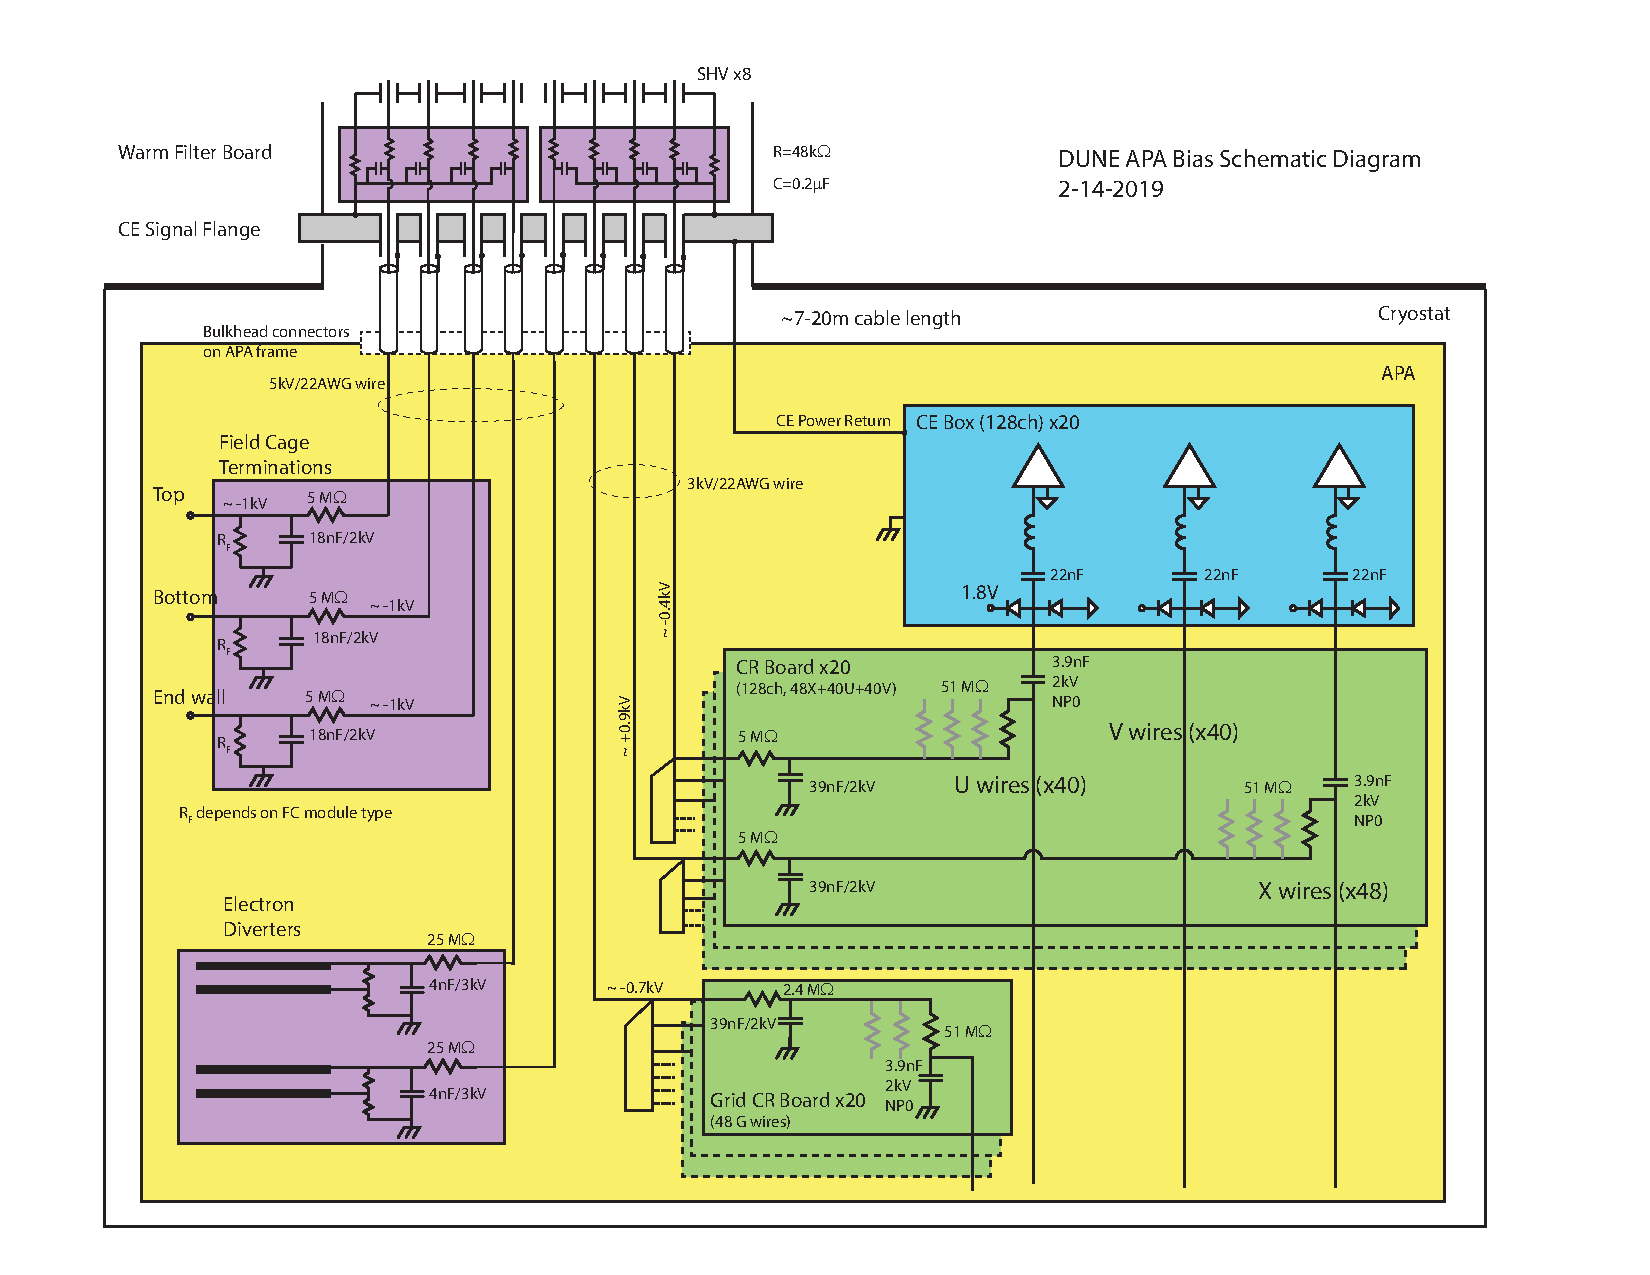
\includegraphics[width=0.8\linewidth]{sp-tpcelec-cr-board.pdf}
\end{dunefigure}

Bias resistance values should be at least \SI{20}{\mega\ohm} to 
maintain negligible noise contributions. The higher value helps 
achieve a longer time constant for the high-pass coupling networks.
Time constants should be at least \num{25} times the electron 
drift time so that the undershoot in the digitized waveform
is small and easily correctable. However, leakage currents can 
develop on \dwords{pcb} that are exposed to high voltages over 
extended periods. If the bias resistors are much greater than 
\SI{50}{\mega\ohm}, leakage currents may affect the bias voltages 
applied to the wires. As discussed in Section~\ref{sec:crboards},
the bias resistance value is \SI{50}{\mega\ohm}, while the 
\dword{dc}-blocking capacitors on each wire have a value of
\SI{3.9}{nF}. This gives a time constant of \SI{0.2}{s} that
is much larger than the drift time for electrons from tracks
passing near the cathode.

The bias-voltage filters are RC low-pass networks. Resistance 
values should be much smaller than the bias resistances to control 
cross-talk between wires and limit the voltage drop if any of the 
wires becomes shorted to the \dword{apa} frame. As discussed
in Section~\ref{sec:crboards}, these resistors are %have a resistance
\SI{2.2}{\mega\ohm}, while the bias filter capacitors are \SI{39}{nF}.

%%%%%%%%%%%%%%%%%%%%%%%%%%%%%%%%%%%
\subsection{Front End Motherboard}
\label{sec:fdsp-tpcelec-design-femb}

Each \dword{apa} is instrumented with \num{20} \dwords{femb}.
The \dwords{femb} plug into the \dword{apa} \dword{cr} boards, 
making the connections from the wires to the charge amplifier 
circuits as short as possible. Each \dword{femb} receives signals 
from \num{40} $U$ wires, \num{40} $V$ wires, and \num{48} $X$ wires.
The baseline \dword{femb} design contains eight \num{16}-channel 
\dword{fe} (\dword{larasic}) \dwords{asic}, eight \num{16}-channel 
\dword{coldadc} \dwords{asic}, and two \dword{coldata} control and 
communication \dwords{asic} (see Figure~\ref{fig:ce-scheme}).
The \dword{femb} also contains regulators that produce the voltages 
required by the \dwords{asic} and filter those voltages, and 
a micro-electromechanical system oscillator that is used to
filter out the jitter from the clock received from the \dword{wib}.
\fixme{previous sentence unclear}
The \dword{larasic} inputs are protected by diodes and a series inductor.

\begin{dunefigure}
[The baseline \dword{ce} architecture.]
{fig:ce-scheme}
{The baseline \dword{ce} architecture. The basic unit is the 
128-channel \dword{femb}. The scheme includes also the 
\dwords{sipm} used for the readout of the \dwords{pd}.}
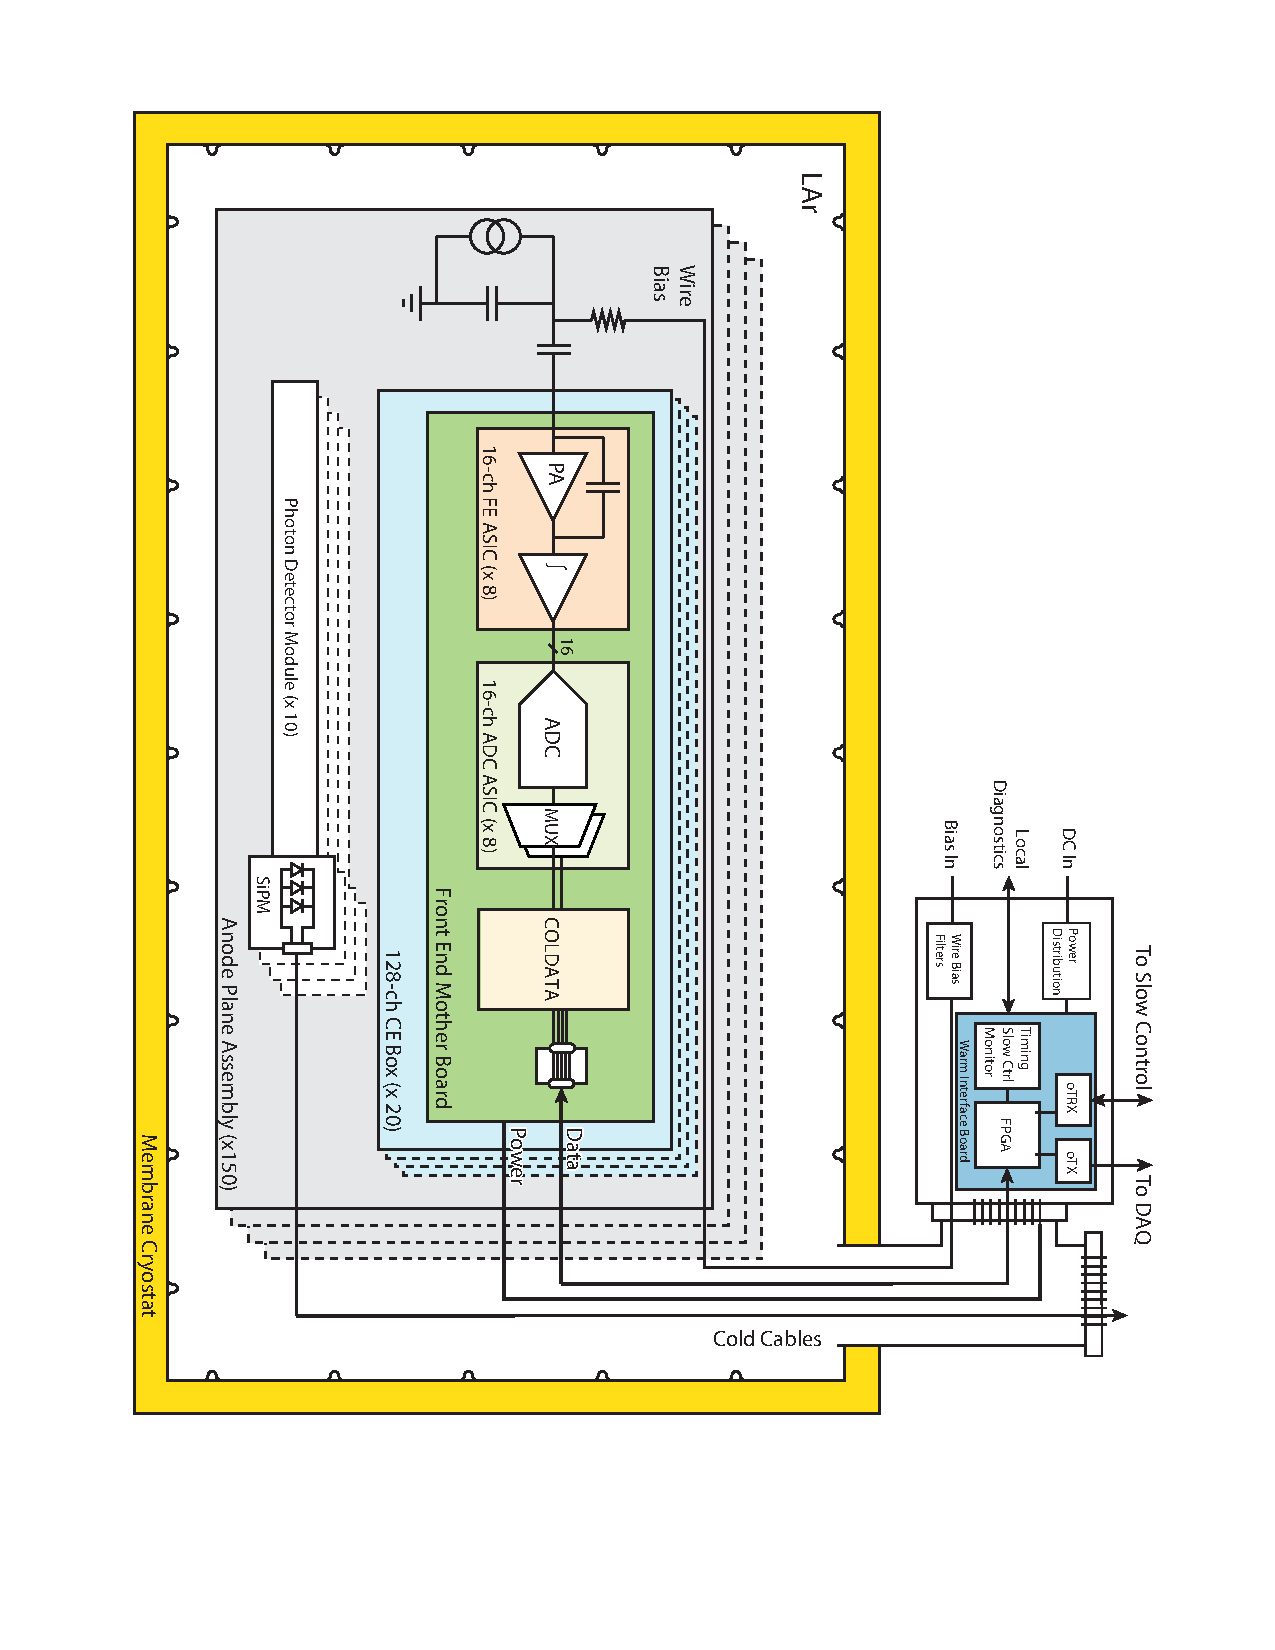
\includegraphics[width=0.99\linewidth]{sp-tpcelec-schematic-v3.pdf}
\end{dunefigure}

The \dword{pdsp} version of the \dword{femb} (which uses a single 
\dword{fpga} on a mezzanine card instead of two \dword{coldata} 
\dwords{asic}) is shown in Figure~\ref{fig:femb}. In the rest of
this section we describe the \dwords{asic} that can be installed
on the \dwords{femb} and discuss the procedure that will be 
followed to choose the \dword{asic} %solution to be implemented for 
to implement in the %\dword{dune} 
\dword{spmod}. % construction. 
In addition to
describing \dword{larasic}, \dword{coldadc}, and \dword{coldata},
we also discuss two alternative solutions, one based on a 
\dword{cots} \dword{adc}, and one where the functionality of the
three \dwords{asic} is implemented in a single chip, \dword{cryo}.

\begin{dunefigure}
[The complete \dword{femb} assembly as used in \dword{pdsp}.]
{fig:femb}
{The complete \dword{femb} assembly as used in the \dword{pdsp} 
detector. The cable shown is the high-speed data, clock, and control cable.}
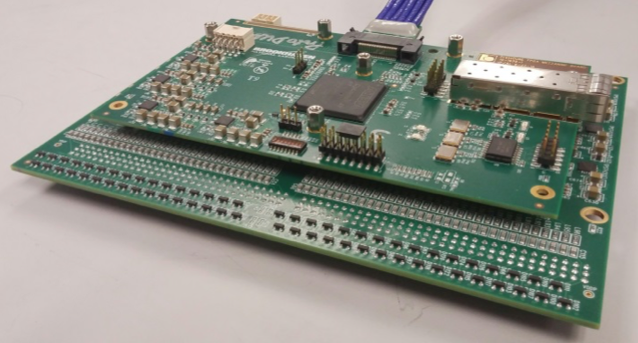
\includegraphics[width=0.6\linewidth]{sp-tpcelec-femb.png}
\end{dunefigure}

The functionality of the \dword{femb} for \dword{dune} will be
almost identical to that of \dword{femb} used in \dword{pdsp}.
The design will change slightly to accommodate the new \dwords{asic},
which will also entail changing the connections to the \dword{wib},
and changing the number of voltage regulators. In addition, the
connector for the control and data cold cables will be replaced
to address the issue observed in \dword{pdsp} that was discussed
in Section~\ref{sec:fdsp-tpcelec-overview-lessons}. The new design,
shown in Figure~\ref{fig:femb-connector}, foresees the addition
of wings to the \dword{pcb} soldered to the cold cable, with 
surface mount standoffs to ensure the planarity of the connector
to the \dword{femb}, and a cutout in the \dword{pcb} to preclude %avoid
any stresses introduced by height variations.

\begin{dunefigure}
[Modified design of the cold data cable and of the \dword{femb} \dword{pcb}.]
{fig:femb-connector}
{Modified design of the cold data cable and of the \dword{femb} \dword{pcb}.}
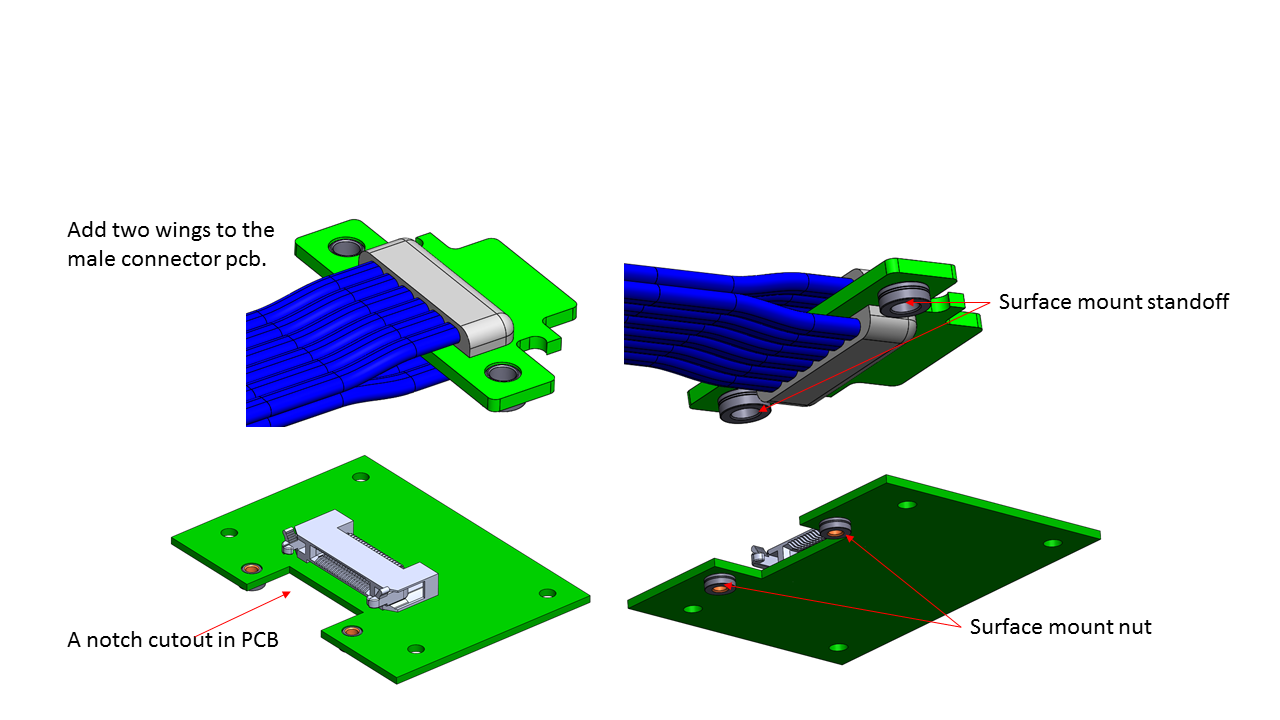
\includegraphics[width=0.9\linewidth]{sp-tpcelec-connector.png}
\end{dunefigure}

All the components on the \dword{femb} need to have a very long lifetime
in \dword{lar}, including commercial resistors and capacitors, the
\dword{lv} regulators, and the micro-electromechanical system oscillator.
In order to achieve the targeted lifetime of \dunelifetime{}, all commercial components 
need to be qualified with %and 
their lifetime in \dword{lar} %need to be 
measured. 
In the case of custom \dwords{asic}, appropriate steps must be taken prior 
to starting the layout of the chips. Both \dword{coldata} and 
\dword{coldadc} are implemented in the \dword{tsmc} \SI{65}{nm} \dword{cmos} 
process~\cite{TSMC65}. The designs were done using cold transistor models 
produced by Logix Consulting\footnote{Logix\texttrademark{} Consulting, http://www.lgx.com/.}.  Logix made measurements of 
\dword{fnal}-supplied \dword{tsmc} \SI{65}{nm} transistors at \lntwo 
temperature and extracted and provided to the design teams \dword{spice} 
models valid at \lntwo temperature.  These models were used in 
analog simulations of \dword{coldata} and \dword{coldadc} subcircuits.  
In order to eliminate the risk of accelerated aging due to the hot-carrier
effect~\cite{Hot-electron}, no transistor with channel length
less than \SI{90}{nm} was used in either \dword{asic} design.
A special library of standard cells using \SI{90}{nm} channel-length 
transistors was developed by members of the University
of Pennsylvania and \dword{fnal} groups. Timing parameters were
developed for this standard cell library using the Cadence Liberate
tool\footnote{Cadence Liberate\texttrademark{}, \url{https://www.cadence.com/content/cadence-www/global/en_US/home/tools/custom-ic-analog-rf-design/library-characterization/liberate-characterization.html}. } 
and the Logix \dword{spice}~\cite{spice} models. With the
exception of the \dword{coldata} \dword{pll}, 
\fixme{PLL is defined as a word not an abbreviation, so it doesn't get written out on first use. Do we want to change this and others like it to abbreviations in the glossary?} 
serializer, and
output driver, the digital sections of \dword{coldata} and
\dword{coldadc} were synthesized from Verilog code using this
standard cell library and the Cadence Innovus tool~\footnote{Cadence Innovus\texttrademark{}, \url{https://www.cadence.com/content/cadence-www/global/en_US/home/tools/digital-design-and-signoff/hierarchical-design-and-floorplanning/innovus-implementation-system.html}.}. 
Innovus was also used for the layout of the synthesized logic.
The design of the \dword{cryo} \dword{asic} and of \dword{larasic}
are implemented in the \dword{tsmc} \SI{130}{nm} and \SI{180}{nm} 
\dword{cmos} process~\cite{TSMC130,TSMC180}, respectively. In the
first case the design is based on \dword{spice} models valid at
\lntwo temperature, that were derived following the same approach
as for the \SI{65}{nm} technology. In the case of \dword{larasic}, 
the design uses models that were obtained by extrapolating the
parameters of the models provided by \dword{tsmc}, which are 
generally valid in the \SIrange{230}{400}{K}.

%%%%%%%%%%%%%%%%%%
\subsubsection{Front End \dword{asic}}
\label{sec:fdsp-tpcelec-design-femb-fe}

The analog \dword{fe} \dword{asic}~\cite{DeGeronimo:2011zz} receives 
current signals from the \dword{tpc} sense wires and provides a way to 
amplify and shape the signals for downstream signal digitization. 
The \dword{fe} \dword{asic} has \num{16} channels and is implemented 
using the \dword{tsmc} \SI{180}{nm} \dword{cmos} process~\cite{TSMC180}. It 
integrates a band-gap reference to generate all the internal bias 
voltages and currents. This guarantees high stability of the operating 
point over a wide range of temperatures, including cryogenic temperatures. 
The channel schematic of the \dword{fe} \dword{asic} is shown in 
Figure~\ref{fig:feasic1}. 

\begin{dunefigure}
[\dword{fe} \dword{asic} channel schematic]
{fig:feasic1}
{Channel schematic of \dword{fe} \dword{asic}, which includes a 
dual-stage charge amplifier and a \num{5}$^{th}$ order semi-Gaussian 
shaper with complex conjugate poles. Circuits in red circles are 
programmable to allow different gain and peaking time settings.}
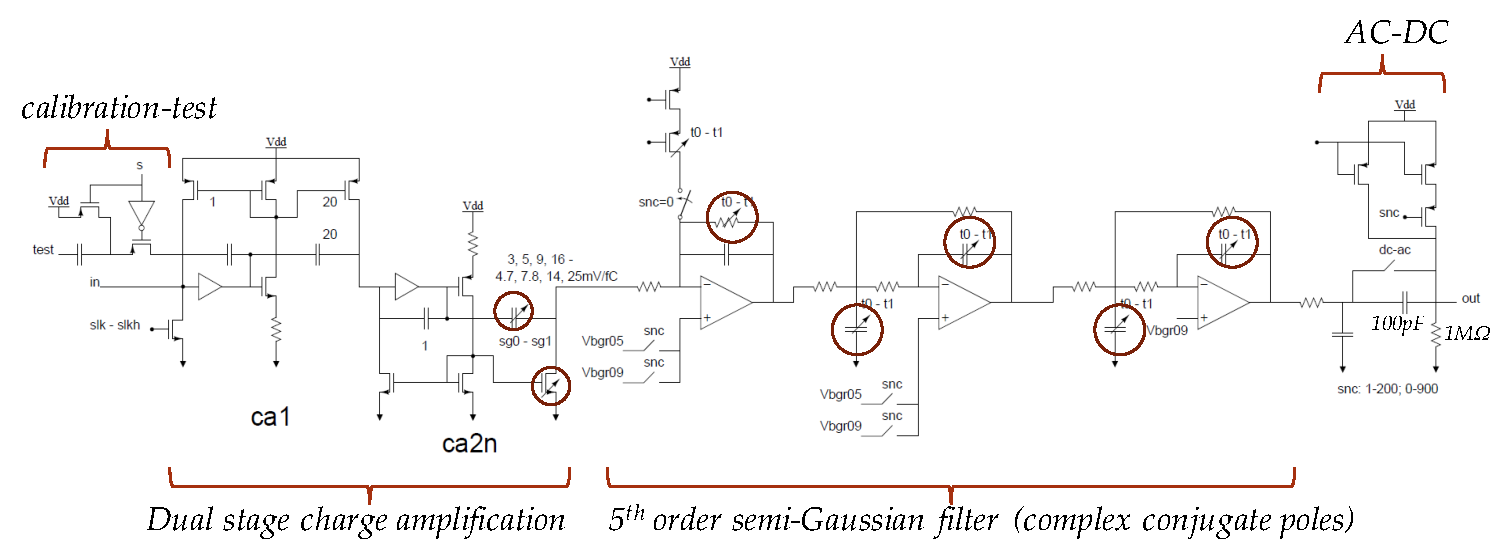
\includegraphics[width=0.99\linewidth]{sp-tpcelec-feasic-channelschematic.pdf}
\end{dunefigure}

Each \dword{fe} \dword{asic} channel has a dual-stage charge amplifier 
and a \num{5}$^{th}$ order semi-Gaussian shaper as an anti-aliasing 
filter for the \dword{tpc} signals. It has a programmable gain 
selectable from one of \num{4.7}, \num{7.8}, \num{14}, or \SI{25}{mV/fC}
(corresponding to full-scale charge of \num{300}, \num{180}, \num{100}, 
and \SI{55}{C}), a programmable peaking time selectable from one of 
\num{0.5}, \num{1}, \num{2}, and \SI{3}{$\mu$s}, and a programmable 
baseline for operation with either the collection ($\sim$\SI{200}{mV}) 
or the induction ($\sim$\SI{900}{mV}) wires. Each channel has an 
option to enable the output monitor to probe the analog signal, and 
an option to enable a high-performance output driver that can be 
used to drive a long cable. 

Each \dword{fe} \dword{asic} channel has a built-in charge calibration 
capacitor that can be enabled or disabled through a dedicated register. 
The injection capacitance has been measured using a calibrated external 
capacitor. The measurements show that the calibration capacitance is 
extremely stable, changing from \SI{184}{fF} at room temperature to 
\SI{183}{fF} at \SI{77}{K}. This result and the measured stability of 
the peaking time demonstrate the high stability of the passive 
components as a function of temperature. Channel-to-channel and 
chip-to-chip variation in the calibration capacitor are typically 
less than \num{1}\%. The variations of the calibration capacitors
could be characterized prior to the beginning of \dword{dune}
data taking, using the \dword{qc} process, discussed in
Section~\ref{sec:fdsp-tpcelec-integration-qc}.

Shared among the \num{16} channels in the \dword{fe} \dword{asic} are 
the digital interface, programming registers, a temperature monitor, 
and a band-gap reference monitor. We also can enable \dword{ac} 
coupling as mitigation of microphonics, a programmable bias current 
selectable from one of \num{0.1}, \num{0.5}, \num{1}, or \SI{5}{nA}, 
as well as a programmable pulser generator with a \num{6}-bit 
\dword{dac} for calibration. The possibility of configuring various
parameters controlling the \dword{fe} amplifier (gain, shaping time,
baseline) has allowed \dword{pdsp} to reduce the impact of the
saturation effect discussed in Section~\ref{sec:fdsp-tpcelec-overview-lessons}, 
at the cost of a reduction in dynamic range.

The power dissipation of \dword{fe} \dword{asic} is about \SI{5.5}{mW} 
per channel at \SI{1.8}{V} supply voltage with output buffer disabled. 
The \dword{asic} is packaged in a commercial, fully encapsulated 
plastic \num{80} pin \dword{qfp}. Figure~\ref{fig:feasic2} shows the 
response of \dword{fe} \dword{asic} for all gains and peaking times 
and both baselines. Note that the gain is independent of the peaking 
time; the same amount of charge produces the same peak voltage signal 
regardless of the peaking time.

\begin{dunefigure}
[\dword{fe} \dword{asic} response and layout]
{fig:feasic2}
{Response of \dword{fe} \dword{asic} for four gains, four peaking times, 
and both baseline values (left); layout of \num{16}-channel \dword{fe} 
\dword{asic} version P3, where revisions with reference to version 
P2 are highlighted in yellow boxes (right).}
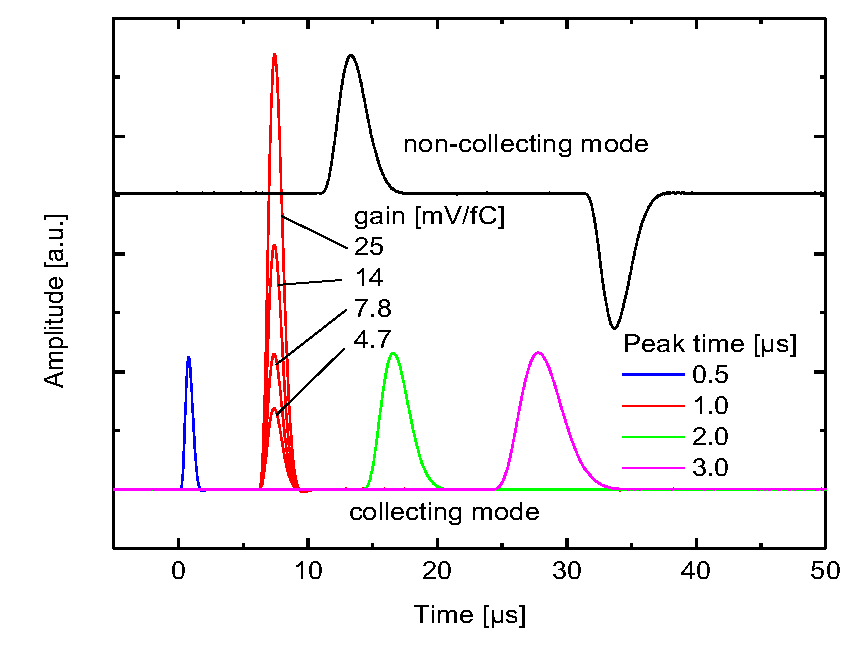
\includegraphics[width=0.53\linewidth]{sp-tpcelec-feasic-response.pdf}
\hspace{6mm}
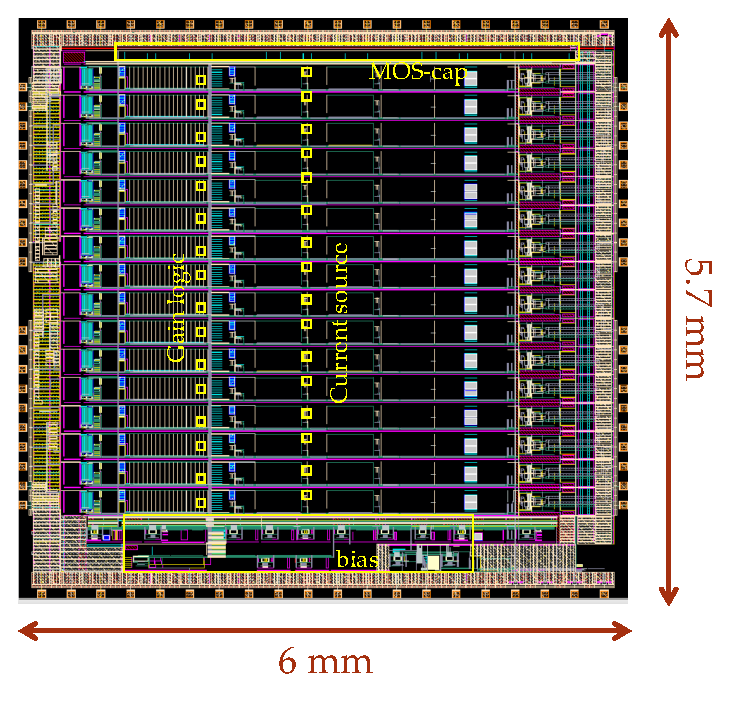
\includegraphics[width=0.42\linewidth]{sp-tpcelec-feasic-layout.pdf}
\end{dunefigure}

Prototype version P2 \dword{fe} \dwords{asic} have been evaluated and 
characterized at room temperature and \lntwo (\SI{77}{K}) temperature. 
\num{960} P2 \dword{fe} \dwords{asic}, totaling \num{15,360} channels, 
have been used to instrument six \dword{pdsp} \dword{apa}s successfully. 
Excessive stress in the package of the \dword{fe} \dword{asic} at cryogenic 
temperature causes \dword{fe} channels to have a non-uniform baseline in 
collection mode, while the baseline \dword{dc} voltage in induction mode 
is uniform. A new prototype, version P3, was fabricated in March 2018 
to address this issue by making \dword{dc} circuits for the collection mode 
similar to the induction mode. At the same time, the default gain
setting was changed to \SI{14}{mV/fC}. The layout of P3 \dword{fe} 
\dword{asic} is also shown in Figure \ref{fig:feasic2}, with modifications 
highlighted in yellow boxes. The P3 \dword{fe} \dwords{asic} were 
received and evaluated in September 2018, and both baseline in collection 
mode and default gain setting are working properly.

P3 \dword{fe} \dword{asic} will be further evaluated on \dwords{femb} 
in various integration test stands for performance studies, including 
the \num{40}\% \dword{apa} at \dword{bnl}, the \dword{iceberg} \dword{tpc} 
at \dword{fermilab} and the seventh \dword{protodune} \dword{apa} 
in the cold box at \dword{cern}. Test results of P3 \dword{fe} \dword{asic} 
will guide the development of the next version P4 \dword{fe} \dword{asic}, 
which will be implemented a single-ended to differential converter for 
interface to recently developed \dword{coldadc}. 
\fixme{I can't parse prev sentence} The P4 version of 
\dword{larasic} will also address the saturation problem observed in
the \dword{pdsp} initial operation, discussed in 
Section~\ref{sec:fdsp-tpcelec-overview-lessons}. The plan for solving
this issue is discussed %below 
in Section~\ref{sec:fdsp-tpcelec-overview-remaining}.

%%%%%%%%%%%%%%%%%%
\subsubsection{\dword{coldadc} \dword{asic}}
\label{sec:fdsp-tpcelec-design-femb-adc}

\dword{coldadc} is a low-noise \dword{adc} \dword{asic} designed to digitize
\num{16} input channels at a rate of \SI{2}{MHz}. It is implemented in the \dword{tsmc}
\SI{65}{nm} \dword{cmos} technology and has been designed by a team of engineers
from \dword{lbnl}, \dword{bnl}, and \dword{fnal}.  The \dword{asic} uses a conservative,
industry-standard design including digital calibration.  Each \dword{coldadc}
receives \num{16} voltage outputs from a single \dword{larasic} chip.  The voltages
are buffered, multiplexed by \num{8}, and input to two \num{15}-stage pipelined \dwords{adc}
operating at \SI{16}{MHz}.  The \dword{adc} uses the well-known pipelined architecture
with redundancy~\cite{PipelinedADC}.  Digital logic is used to correct non-linearity
introduced by non-ideal amplifier gain and offsets in each pipeline
stage~\cite{CalibrationCorrection}, and an automatic calibration procedure is
implemented to determine the constants used in this logic.  The \dword{adc} produces
\num{16}-bit output which is expected to be truncated to \num{12} bits.

The \dword{adc} is highly programmable to optimize performance at different
temperatures.  In order to maximize the probability that the first prototype
\dword{coldadc} will perform well, many circuit blocks can be bypassed. A block
diagram of the chip is shown in Figure~\ref{fig:COLDADC_Block_Diagram}. Each of
the major blocks is described below.

\begin{dunefigure}
[\dword{coldadc} block diagram]
{fig:COLDADC_Block_Diagram}
{\dword{coldadc} block diagram}
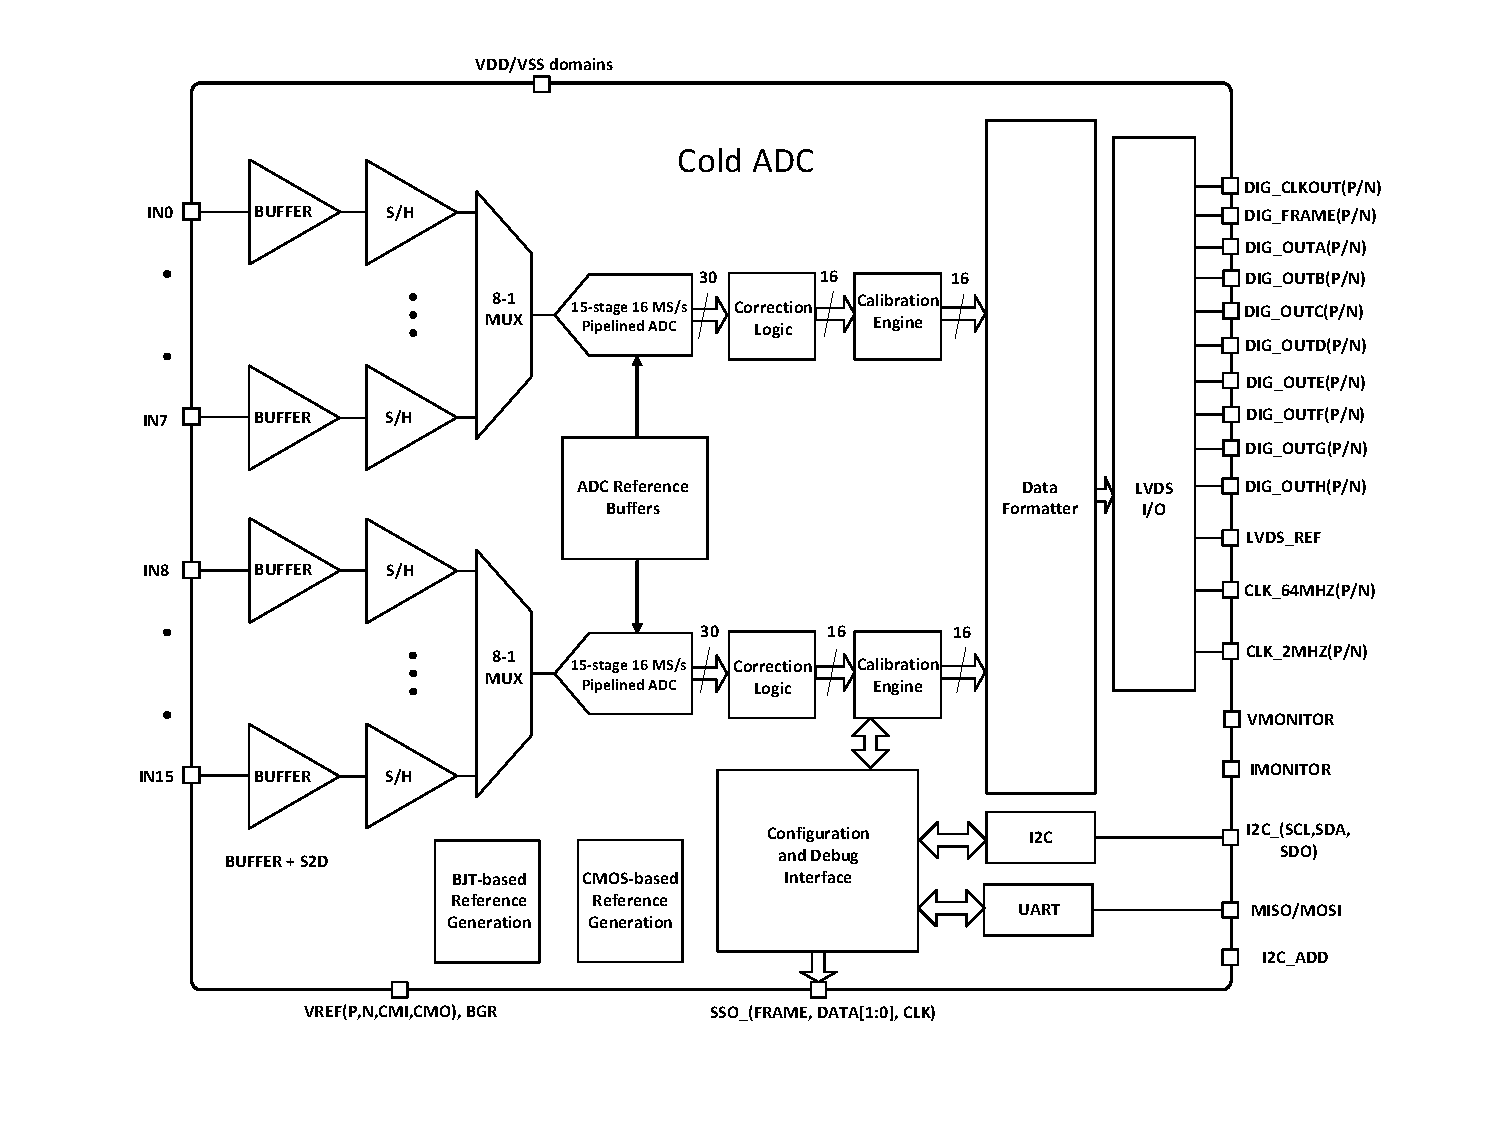
\includegraphics[width=0.8\linewidth]{sp-tpcelec-COLDADCblockdiagram.pdf}
\end{dunefigure}

All required reference voltages and currents are generated on-chip by programmable
circuit blocks. The most accurate reference voltage circuit is a band-gap reference
based on a \dword{pnp} transistor.  However, measurements made at \dword{bnl} and
\dword{lbnl} of a large \dword{pnp} transistor indicate that the foundry-provided \dword{spice} model
does not adequately describe the device operation at \lar temperature.  Thus,
a \dword{cmos}-based voltage reference has also been included in \dword{coldadc}.
In the event that both on-chip reference generation circuits fail, an external voltage
reference can be used.

Independently adjustable bias voltage levels and currents are provided for the
input buffers, sample-and-hold amplifiers, \dwords{adc}, and \dword{adc}
reference buffers.

\dword{coldadc} has four possible ways to interface with \dword{larasic}.  It
can accept either single-ended inputs (provided by existing \dword{larasic}
chips) or differential inputs (foreseen for the future \dword{larasic} P4 upgrade).
In either case, to mitigate the risk that the input buffer circuits do not perform
well, it is also possible to bypass the input buffers and apply the inputs directly
to the sample-and-hold amplifiers.  The sample-and-hold amplifiers are separated
into two groups of eight.  They sample the waveform at the rising edge of the
(\SI{2}{MHz}) sampling clock.  An internally generated \SI{16}{MHz} clock is then
used to clock an \num{8}-to-\num{1} multiplexer that presents eight samples in 
turn to one of the two \dword{adc} pipelines.

A block diagram of an \dword{adc} pipeline is shown in
Figure~\ref{fig:pipelinestage}. Each of the \num{15} stages contains a low-resolution
\num{1.5}-bit analog-to-digital subconverter containing two comparators, a
\num{1.5}-bit digital-to-analog subconverter that produces a voltage based on
the two comparator outputs, an analog subtractor, a sample-and-hold amplifier,
and a gain stage (with a nominal gain of two). The transfer function of
each stage is identical and is shown in Figure~\ref{fig:ADCXFERFN} along with
the nominal ``weights'' (W$_0$ and W$_2$) that are added to form the output of the
pipeline. Each pipeline stage makes a three-level coarse decision based on the
analog input voltage, selects one of three digital ``weights'' to be added to the
results of previous stages, and passes a voltage to the next stage that is
proportional to the difference between the input voltage and the voltage
corresponding to the digital output of the stage.  Because the stages are
weighted by a factor of two, but have three possible digital results, there is
redundancy between stages that makes the final result independent of errors in
the comparator thresholds (up to $\pm V_r/4$ where the stage range is
$[-V_r,V_r]$).  An ``error'' in the output of one stage is corrected in subsequent
stages (usually the next stage).  In order to take advantage of this redundancy
provided by the pipelined architecture it is necessary to include at least one
``extra'' stage in the pipeline.  The \dword{coldadc} pipelined \dwords{adc} are
implemented as \num{15}-stage pipelines.

\begin{dunefigure}
[Circuit blocks in each \dword{adc} pipeline stage]
{fig:pipelinestage}
{Circuit blocks in each \dword{adc} pipeline stage. MUX is circuit that controls
which weight is applied to the result of the previous stage, that is then subtracted
in the ADD circuit from the input of the previous stage. SHA is a sample and hold and
ADCS and DASC are low resolution 1.5 bit analog-to-digital and digital-to-analog 
subconverters, respectively.}
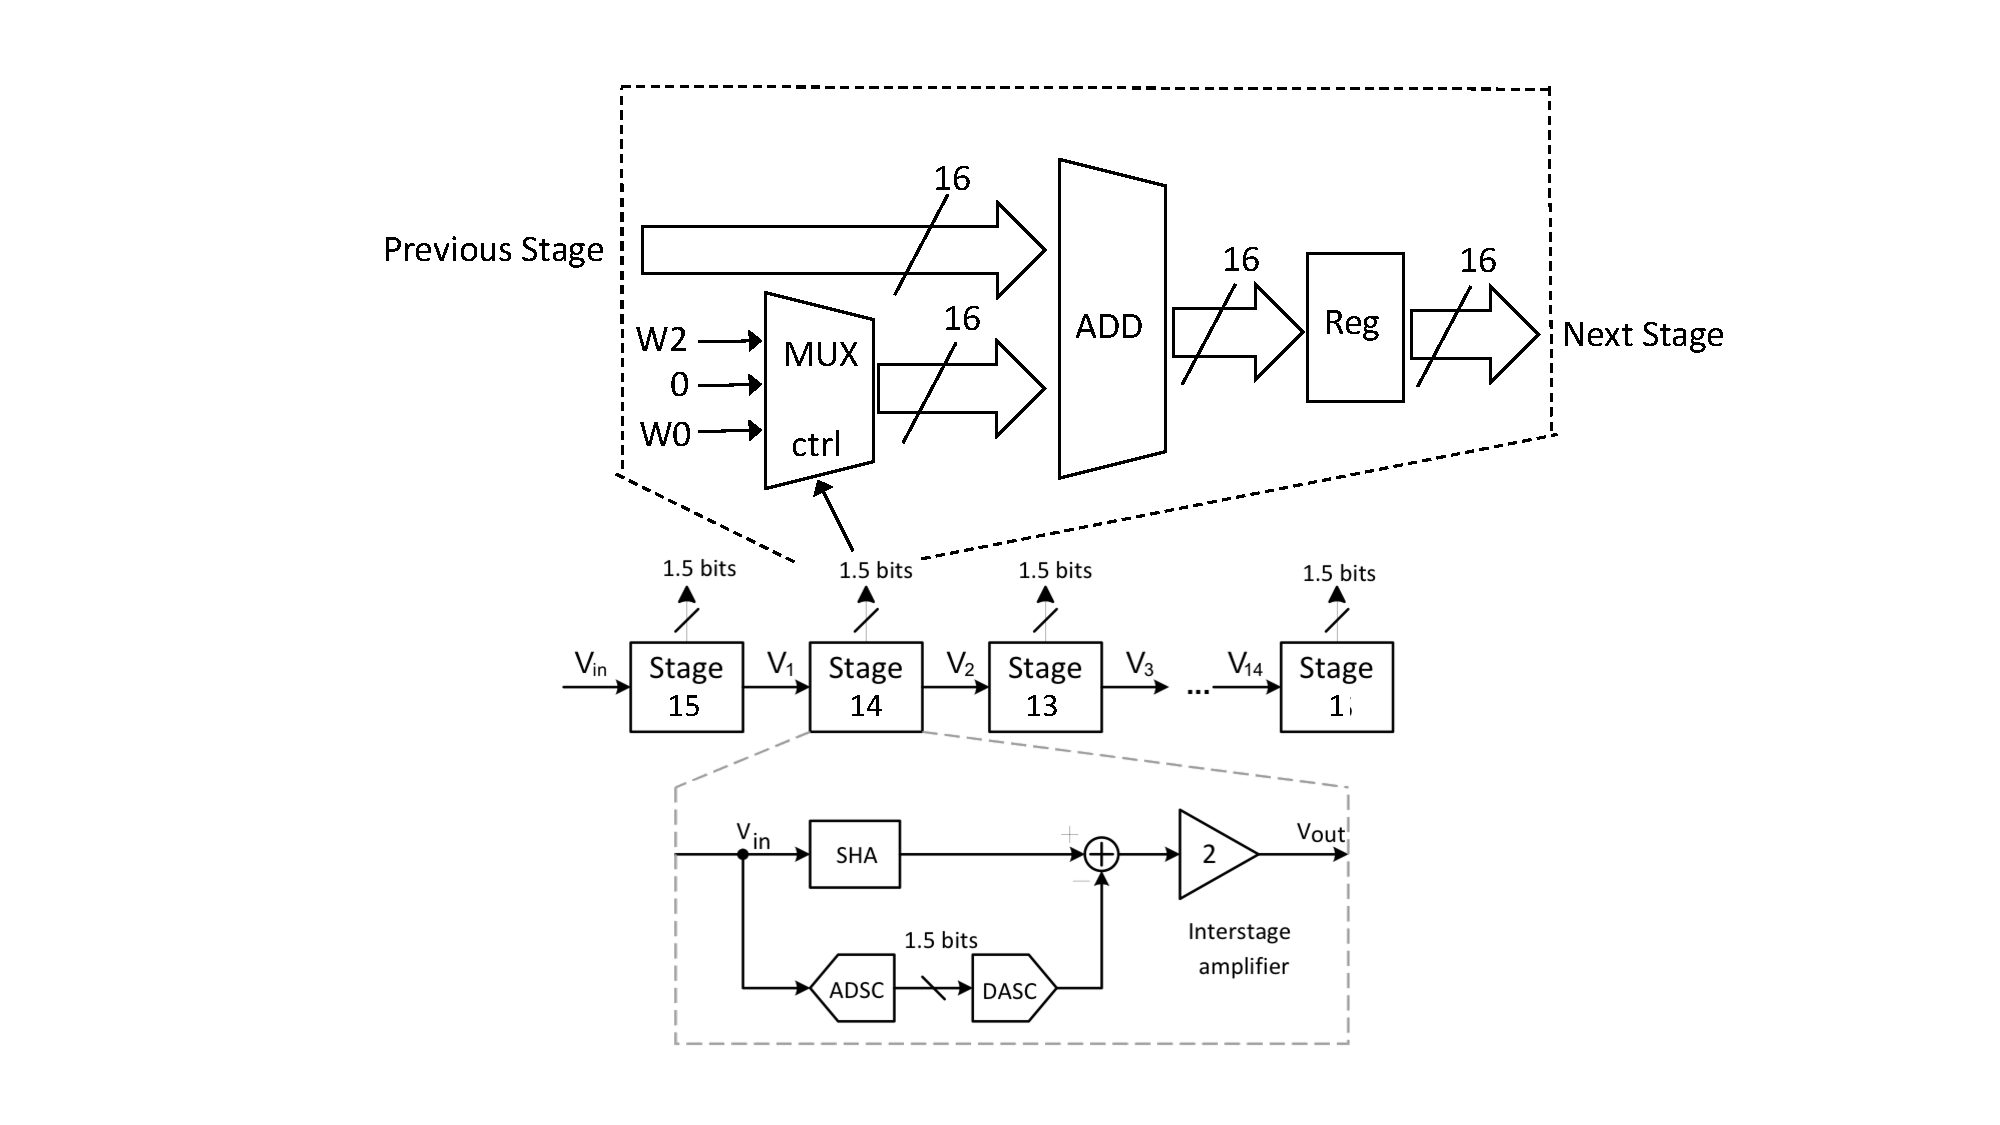
\includegraphics[width=0.9\linewidth]{sp-tpcelec-Pipelinestage.pdf}
\end{dunefigure}

\begin{dunefigure}
[ADC stage transfer function]
{fig:ADCXFERFN}
{\num{1.5}-bit stage transfer function and digital output. The voltage 
range of the \dword{adc} as a whole, and of each individual stage 
is $[-V_r,V_r]$.  Note that the voltage passed to the subsequent 
stage will not exceed the stage range even if a comparator threshold 
is wrong by up to $V_r/4$.}
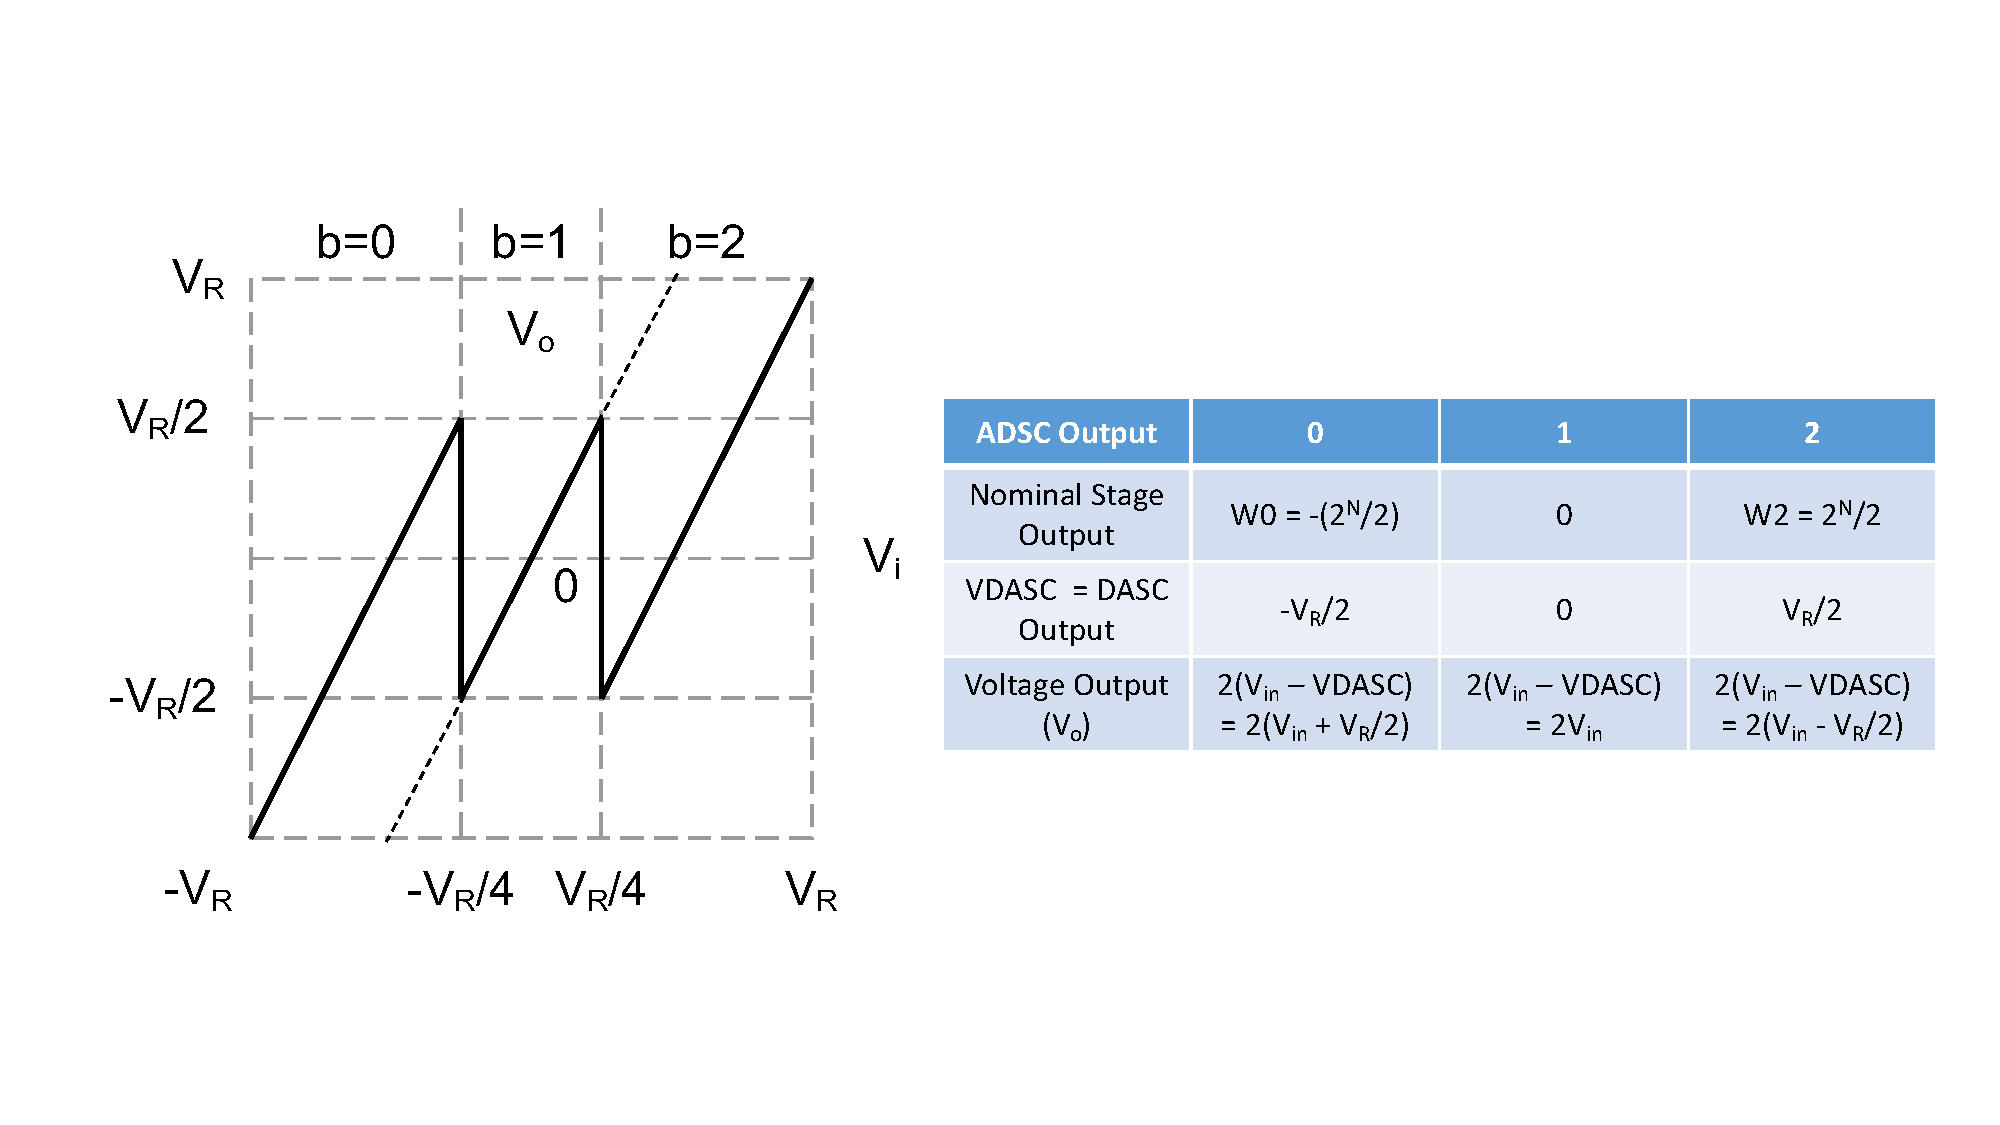
\includegraphics[width=1.0\linewidth]{sp-tpcelec-ADCXFERFN.pdf}
\end{dunefigure}

The calibration logic allows the correction of errors caused by imperfections
in the voltage that are passed from one stage to the next.  These arise from
errors in the voltage in each stage corresponding to $\pm V_r/2$
(generated by resistive dividers) and imperfections in the gain and offset of
the interstage amplifiers.  The calibration procedure relies on the fact that
the required precision is easily satisfied by the last stages of the pipeline.
The number of stages to be calibrated (maximum \num{7}) is set by a programmable
register.  An iterative calibration procedure is used.  Starting with the least
significant stage to be calibrated, the input to the stage is set to the threshold
levels of $\pm V_r/4$ and the normal comparator outputs are overridden
and forced first to \num{1} and then to \num{0}.  The lower stages of the \dword{adc} digitize
the analog value output from the stage being calibrated and the difference between
the \dword{adc} output when the comparator is forced to \num{1} and the \dword{adc}
output when the comparator is forced to \num{0} is calculated.  These two differences
(W$_0$ expressed as a negative number and W$_2$ expressed as a positive number) are
stored and used as two of the three possible digital outputs of the stage being
calibrated (the third possible output being \num{0}).  This procedure is then repeated
for the next most significant pipeline stage until stage \num{15} has been calibrated.

The main weakness of the \num{1.5}-bit per stage pipeline architecture as presented
is that it requires a precise interstage gain of two.  If the gain is greater
than two, then when the input voltage to a stage is close enough to the limits
of the voltage range of the stage, the voltage passed to the next stage will be
out of range.  This will result in skipped \dword{adc} codes.  For this reason,
the interstage gain of \dword{coldadc} is designed to be $\sim$\num{1.998}.  The
calibration procedure recovers the linearity that would be lost due to
non-binary stage weighting.  A small number of \dword{adc} codes near two
extremes of the voltage range are unused, but no skipped codes appear in the
range of codes used. Simulations of \dword{coldadc} including layout parasitics 
indicate that $\sim$\num{150} \num{16}-bit codes will be used at the extremes.
The number of \dword{adc} bits that are useful depends on the effective
noise of the various subcircuits of the \dword{adc}.  The noise of the first few
pipeline stages (associated with the most significant bits) contributes more
heavily than subsequent stages.  For this reason, the first stages are designed
to be larger, lower noise, and to require more power than later stages.  The total
effective noise expected is \SI{\sim130}{$\mu$V}-rms.  This is similar to the
quantization error of an ideal \num{12}-bit \dword{adc} with a voltage range of
\SI{1.5}{V} for which the bin width is \SI{366}{$\mu$V} and the quantization
error is \SI{\sim106}{$\mu$V}.

In normal operation, each pipelined \dword{adc} passes a \num{16}-bit result to the
data formatter on the rising edge of the \SI{16}{MHz} clock.  The data formatter
separates the two \num{16}-bit words into eight \num{4}-bit nibbles and serializes the
nibbles for output (most significant bit first) at \SI{64}{MHz}.  
\fixme{nibbles?} An output
clock and a frame marker are also generated.  The frame marker indicates the most
significant bit in each nibble of the first of eight channels digitized by one
of the \dword{adc} pipelines in each \SI{2}{MHz} sample period.  The output data
is generated on the falling edge of the output clock and is latched by the
\dword{coldata} \dword{asic} using the rising edge of the same clock.  

A second
mode of operation is included for debugging purposes.  In this mode, \num{2}-bit raw
stage results from each of the \num{15} stages of one of the two pipelines are formatted
into the most significant \num{15} bits of two \num{16}-bit words, broken into nibbles, and
output in the same manner as normal data.

Ten differential output drivers are used for the \SI{64}{MHz} output clock, frame
marker, and \dword{adc} data.  The output drivers source and sink a current whose
value can be digitally controlled.  The minimum current is \SI{165}{$\mu$A},
which corresponds to approximately \SI{3}{mV} peak-to-peak with \SI{100}{$\Omega$}
termination.  Seven additional levels spaced by \SI{275}{$\mu$A} can be selected.
The maximum current is \SI{2.07}{mA}, about \num{2/3} of the \dword{lvds} standard of
\SI{3.5}{mA}.

The operation of \dword{coldadc} is controlled by a number of \num{8}-bit registers.
These registers can be written to and read back using either an \dword{i2c}
interface~\cite{bib:I2C} or a \dword{uart}. \dword{coldata} will use the \dword{i2c} interface.  The
\dword{uart} is included in the first \dword{coldadc} prototype to facilitate chip testing
and for risk mitigation.

\metainfo {Results of bench tests (and later system tests in \dword{lar}) will be included
when they are available.  These will include measurements of performance and
also power consumption.}

%%%%%%%%%%%%%%%%%%
\subsubsection{COLDATA \dword{asic}}
\label{sec:fdsp-tpcelec-design-femb-coldata}

The \dword{coldata} \dword{asic} was designed by engineers from \dword{fermilab} 
and Southern Methodist University. It is responsible for all communications 
between the \dwords{femb} and the electronics located outside the cryostat. 
Each \dword{femb} contains two \dword{coldata} chips. \dword{coldata} receives 
command-and-control information from a \dword{wib}. Each \dword{coldata} provides 
clocks to four \dword{coldadc}s and relays commands to four \dword{larasic} 
\dword{fe} \dwords{asic} and four \dword{coldadc}s to set operating modes and 
initiate calibration procedures.  Each \dword{coldata} receives data from four 
\dword{coldadc}s, merges the data streams, provides 8b/10b encoding, serializes 
the data, and transmits the data to the warm electronics over two \SI{1.28}{Gbps} 
links.  These links are driven by line drivers with programmable pre-emphasis. 
Figure~\ref{fig:coldata_block_diagram} is a block diagram of \dword{coldata}. 
The possibility of transmitting data from \dword{coldata} over a single 
\SI{2.56}{Gbps} link will be investigated in 2019, with the goal of further
reducing the number of cold cables that need to be routed through the
\dword{apa} frame, as discussed in Section~\ref{sec:fdsp-tpcelec-interfaces-apa}.

\begin{dunefigure}
[\dword{coldata} block diagram]
{fig:coldata_block_diagram}
{\dword{coldata} block diagram}
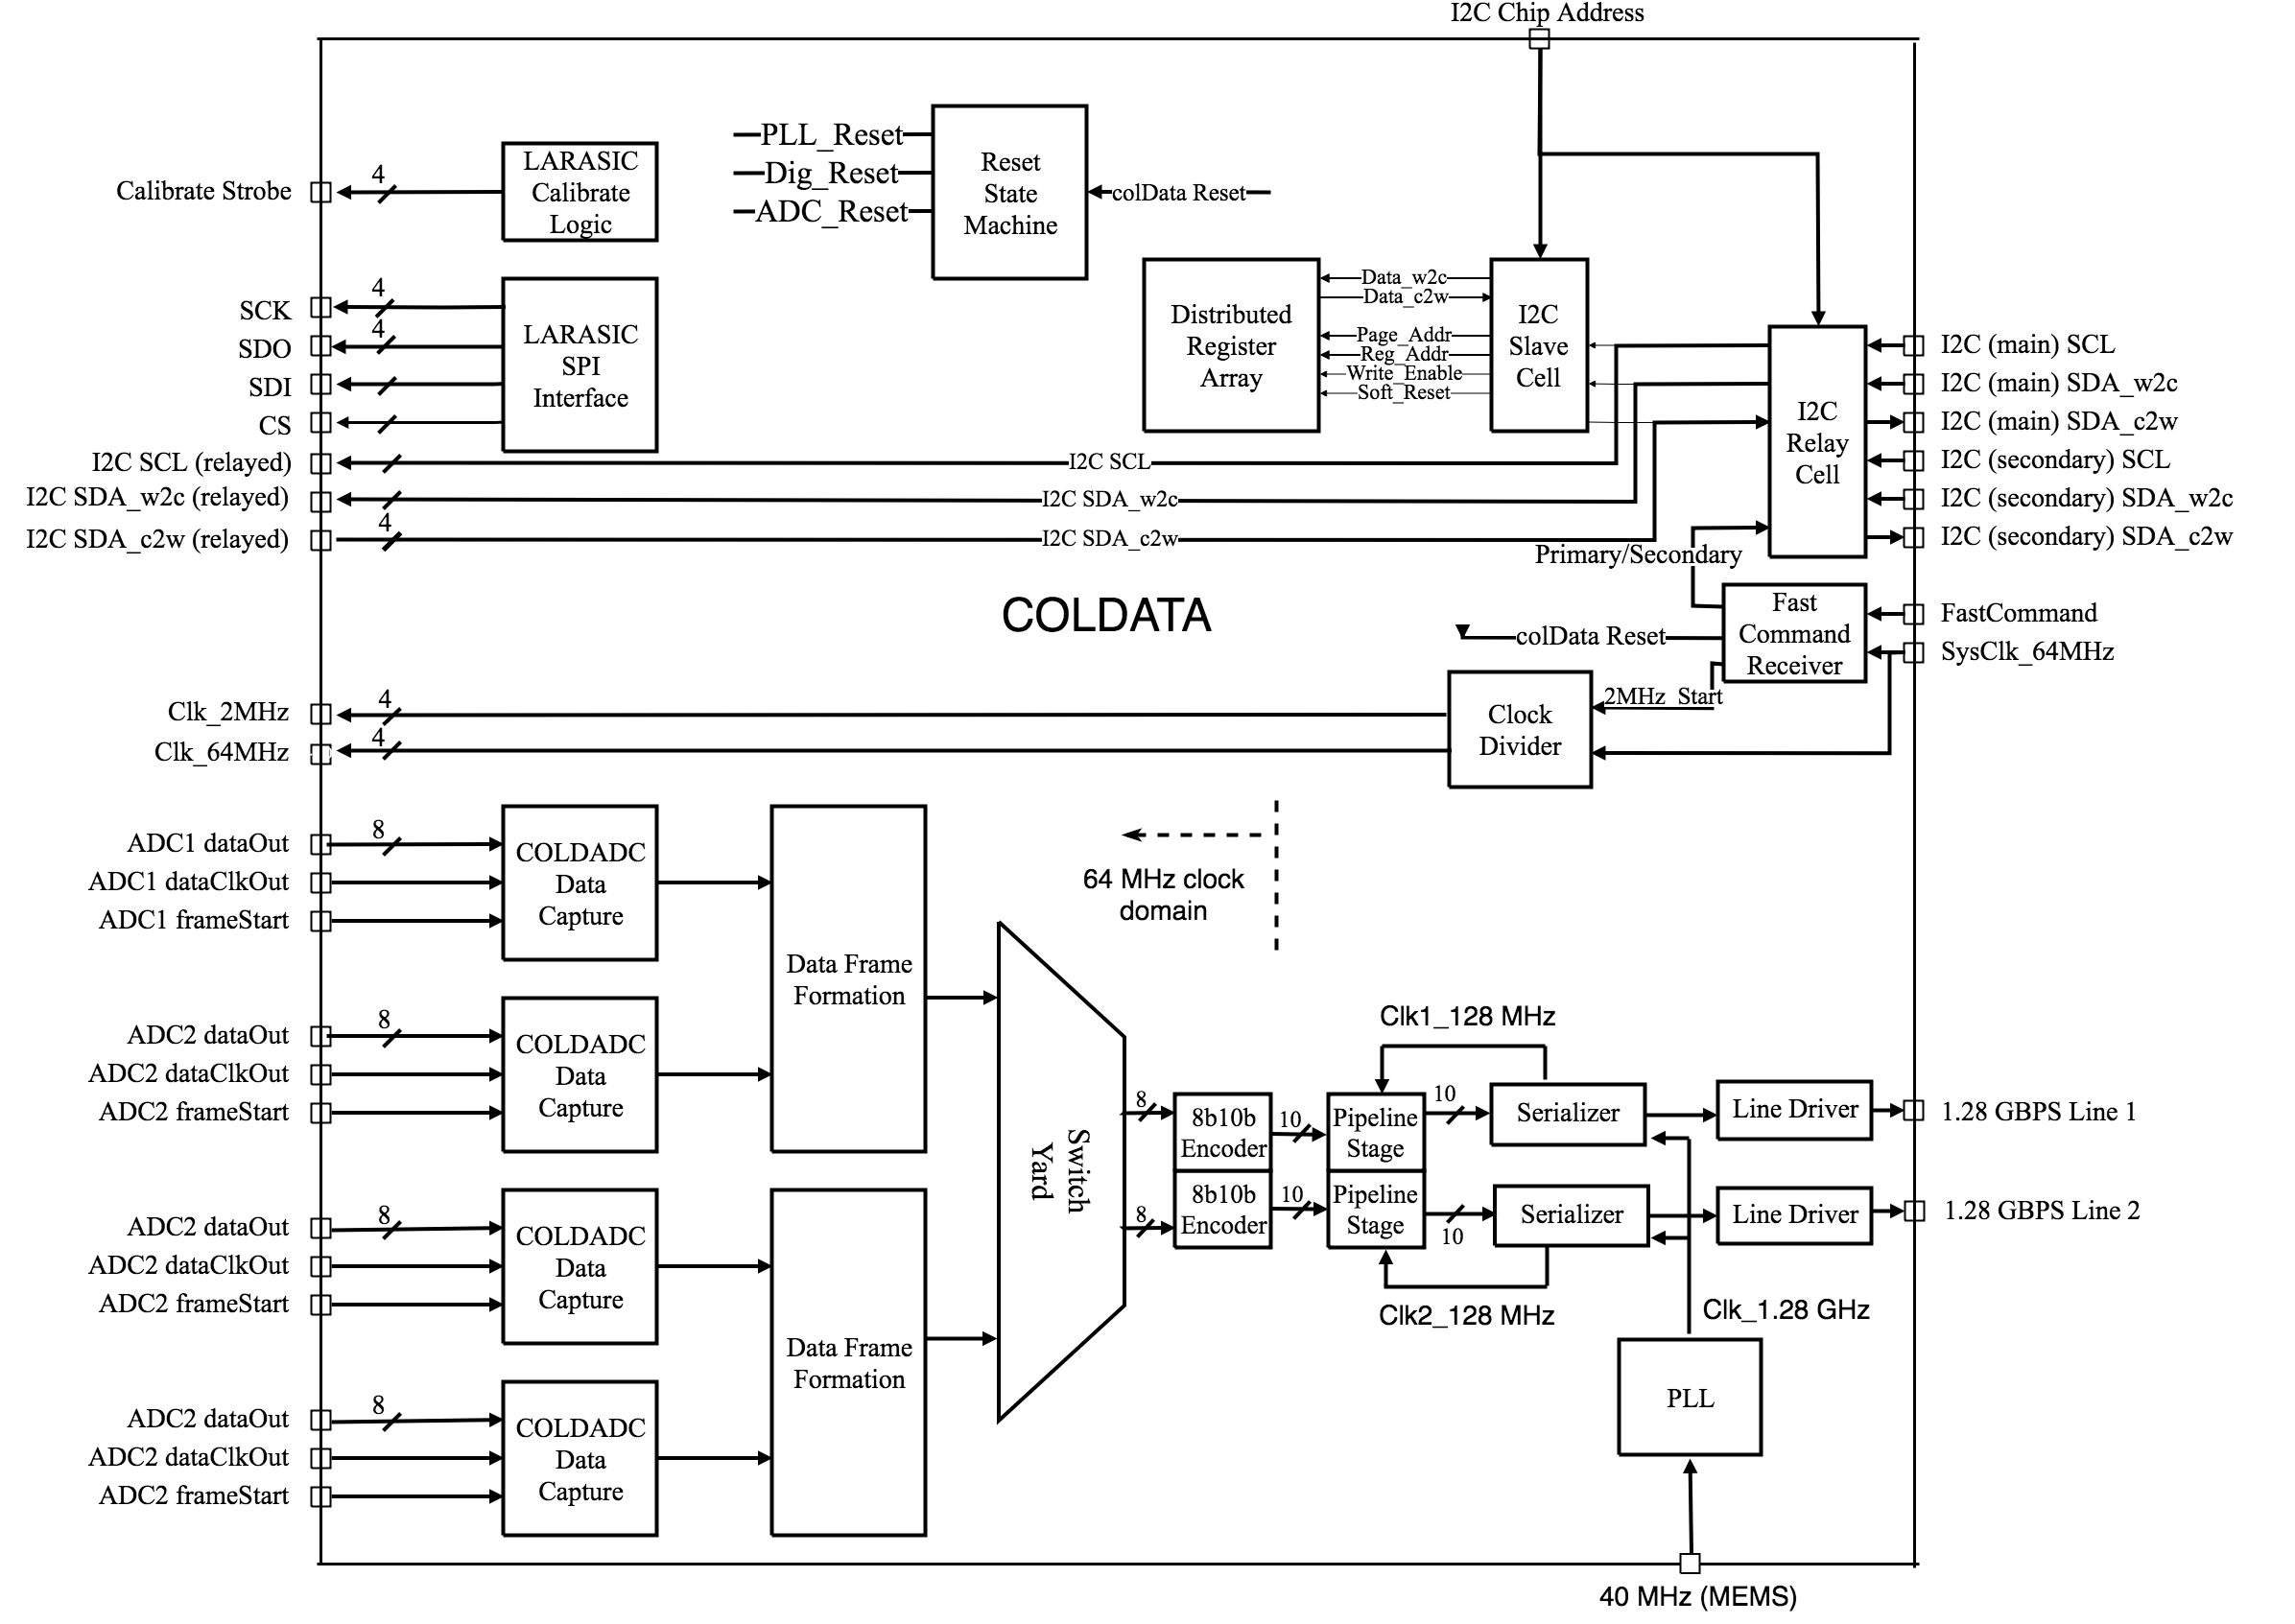
\includegraphics[width=0.9\linewidth]{sp-tpcelec-COLDATA-block-diagram.png}
\end{dunefigure}
\fixme{text on figure is too small and the grey is too light (anne)}

The commands for the control of all the \dwords{asic} on a \dword{femb} are sent 
from a \dword{wib}  
using an \dword{i2c}-like~\cite{bib:I2C} protocol. While standard 
\dword{i2c} uses single-ended \dword{cmos} signals and a bidirectional data 
line, because of the long cables required between the \dword{wiec} and the 
\dwords{femb}, \dword{coldata} uses \dword{lv} differential pairs for both 
the \dword{i2c} clock and data. Point-to-point links are used and separate 
links are used for data sent from warm-to-cold and for data sent from cold-to-warm.  \fixme{the separate links ARE the point to point ones, right?}
In order to reduce the number of cables required, only one of the two 
\dword{coldata} chips on an \dword{femb} has its main \dword{i2c} interface 
directly connected to a \dword{wib}. That \dword{coldata} chip relays \dword{i2c} 
commands and data to the secondary \dword{coldata} chip and relays \dword{i2c} 
responses from the secondary \dword{coldata} to the \dword{wib}. Each 
\dword{coldata} also relays \dword{i2c} commands and data sent from the 
\dword{wib} to one of the four \dword{coldadc} chips associated with that 
\dword{coldata}, as well as data sent back to the \dword{wib} from one of the 
four \dword{coldadc} chips. 
\fixme{IOW (from ``as well as''): and it relays data sent back to the \dword{wib} from one of the four \dword{coldadc} chips TO WHERE?}. 
The links on the \dword{femb} between \dword{coldata} 
chips and \dword{coldadc} chips use single-ended (\SI{2.25}{V}) \dword{cmos} 
signals, but the \dword{i2c} links are still non-standard since  %as separate signals are used for 
data sent to the \dwords{coldadc} and data sent from the 
\dwords{coldadc} to \dword{coldata} are in separate signals. \fixme{check above}

The controls intended for the \dword{larasic} \dword{fe} chips are interpreted 
inside \dword{coldata} and transmitted to the appropriate \dword{asic} using 
a \dword{spi}-like interface that uses single-ended (\SI{1.8}{V}) \dword{cmos} 
signals. The configuration registers in \dword{larasic} are configured to be 
loaded as a single-shift register. As data is shifted into \dword{larasic} on 
the \dword{mosi} line, bits from the other end of the shift register are shifted 
out on the \dword{miso} line. It is thus only possible to read \dword{larasic} 
configuration registers while writing new configuration data.

In addition to the configuration commands, \dword{coldata} %also 
receives a master clock and a fast command signal on a \dword{lv} 
differential pair from
the \dword{wib}. Currently the master clock is \SI{64}{MHz}, but it will be
changed to \SI{62.5}{MHz} to simplify the overall \dword{fd} \dword{spmod} 
synchronization. The clock used for sampling the \dword{adc} is created inside
\dword{coldata} by dividing the master clock by \num{32}. Both the master clock and
the \dword{adc} sampling clocks are passed from \dword{coldata} to the four
\dword{coldadc} chips that it controls. Depending on the master clock frequency
the \dword{adc} will convert input data every \num{500} or \SI{512}{ns}, 
corresponding to a frequency of \num{2}, or \SI{1.95}{MHz}. Signals that must be executed at a known time use the fast command 
line. \dword{coldata} 
uses the falling edge of the master clock to sample fast command bits as shown 
in Figure~\ref{fig:coldata_fast_command_timing}. All legal fast commands 
are \dword{dc} balanced. An ``alert'' pattern is used to establish the 8-bit 
fast-command word boundary. An ``idle'' pattern is used when no command is being 
sent. Four commands are defined: ``Edge,'' which moves the rising edge of the 
\dword{adc} sampling clock to coincide with the next rising edge of the 
master MHz clock; ``Sync,'' which zeros the \num{8}-bit timestamp that is the incremented 
on the rising edge of each \dword{adc} sampling clock; ``Reset,'' which resets 
\dword{coldata}; and ``ACT,'' the function of which is determined by an \num{8}-bit 
register that is programmed using the \dword{i2c} interface.  

\begin{dunefigure}
[\dword{coldata} fast command timing]
{fig:coldata_fast_command_timing}
{Fast command timing: the leading edges of the fast command and of the master 
clock are equal time when produced on the \dword{wib}. The fast-command bits 
are captured by \dword{coldata} on the falling edge of the master clock and 
shifted into a register on the next positive edge.}
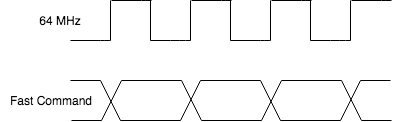
\includegraphics[width=0.4\linewidth]{sp-tpcelec-clocksandfastcommand.png}
\end{dunefigure}

\dword{coldata} receives digitized waveform data from 
four \dword{coldadc} \dwords{asic}. Each \dword{adc} presents its data on eight 
serial streams operating in parallel. Data from the \dwords{adc} is captured 
using the \dword{adc} dataClkOut 
\fixme{signal type? add to glossary?} 
(one per \dword{adc}) and the start of a 
sample period is indicated by the frameStart signal (one per \dword{adc}). 
Each \dword{adc} digitizes \num{16} channels of information and puts out \num{16} bits 
of data per channel. Information from two \dwords{adc} are merged by a Data 
Frame Formation block.  \fixme{Do these terms need to be capitalized? add to glossary?} 
The Data Frame Formation circuitry converts the two 
groups of sixteen \num{16}-bit words into one of three types of data frame. For normal 
data taking, either a \num{12}-bit format or a \num{14}-bit \dword{adc} format can be 
selected, discarding either the four or two lowest order bits. When the 
\num{12}-bit format is selected, a data frame consists of an 8b/10b command 
character (K28.2) and an \num{8}-bit time stamp, followed by \num{48} bytes of \dword{adc} 
data and two bytes of parity information. When the \num{14}-bit format is selected, 
a data frame consists of an 8b/10b command character (K28.3) and an \num{8}-bit time 
stamp, followed by \num{56} bytes of \dword{adc} data and two bytes of parity 
information. Two debugging frame formats are also defined. When the ``Frame-12 Test'' 
format is selected, a data frame consists of an 8b/10b command character 
(K28.0) and an \num{8}-bit time stamp, followed by \num{48} bytes of predefined data 
and two bytes of parity information. The final format is used when the 
\dwords{coldadc} are read out in debug mode. In this case, \num{30} bits of raw 
pipeline stage data are read out from one of the two pipelined \dwords{adc} 
in each \dword{coldadc} \dword{asic} and passed from \dword{coldadc} to 
\dword{coldata} using two \num{16}-bit frames. When the ``Frame-15'' format is 
selected, a \dword{coldata} output data frame consists of an 8b/10b command 
character (K28.6) and an \num{8}-bit time stamp, followed by \num{60} bits of \dword{adc} 
data (\num{30} bits from each \dword{coldadc}). No parity information is generated 
when this format is selected. This is to ensure that at least one idle 
character (K28.1) will be sent between each ``Frame-15.'' A series of 8b/10b 
command characters (K28.5) is sent at the end of each frame of \num{12}-bit or 
\num{14}-bit data to ensure synchronization of the high-speed links.

The serializers and output drivers use clocks derived from a micro-electromechanical
system oscillator on the \dword{femb}. A single \dword{pll} generates a 
\SI{1.28}{GHz} clock for both serializers and output drivers. The \num{10}-bit
serializers are implemented using two \num{5}:\num{1} multiplexers (clocked at \SI{128}{MHz}) 
followed by a single \num{2}:\num{1} multiplexer (clocked at \SI{640}{MHz}). Each serializer 
derives the \SI{640}{MHz} and \SI{128}{MHz} clock from the \SI{1.28}{GHz} 
clock provided by the \dword{pll} and provides its \SI{128}{MHz} clock to 
the Data Frame Formation block, which uses it at the output stage of a 
clock-domain-crossing \dword{fifo}. A link synchronization sequence of 8b/10b 
command characters (K28.5) is used when the link is reset to establish the 
boundary between \num{10}-bit ``words.'' Idle characters (K28.1) are inserted 
by the Data Frame Formation block when no data is ready for serialization 
(between data frames). The \SI{1.28}{Gbps} output drivers include programmable 
pre-emphasis. The pre-emphasis is achieved using a combination of a voltage 
mode circuit at the input to the current mode driver and current mode 
pre-emphasis integrated into the driver circuit. Measurements were made 
of the insertion loss (``S parameters'') as a function of frequency using
\num{25} and \SI{35}{m} lengths of the twinax cable identical to the 
cable used in \dword{pdsp}, and the output driver circuit including 
pre-emphasis was simulated using a \dword{spice} model based on these 
measurements. The simulated eye diagram after \SI{25}{m} of warm twinax 
cable is shown in Figure~\ref{fig:128Gbpseyesim}. The \dword{pll} and 
serializer circuits used in \dword{coldata} were included in the first partial prototype (CDP1) 
test chip that was produced in Fall 2017 and shown to work as designed. \fixme{later it says it was produced in 2018, around line 1657 in this file}
The pre-emphasis circuit has been added to the current mode driver, which 
was verified in CDP1 and can be disabled if desired. 

\begin{dunefigure}
[\dword{coldata} output simulated eye diagram]
{fig:128Gbpseyesim}
{Simulated eye diagram after \SI{25}{m} of \dword{pdsp} twinax at room 
temperature for the \dword{coldata} \SI{1.28}{Gbps} output link.  
The eye diagram is more open at cryogenic temperature.}
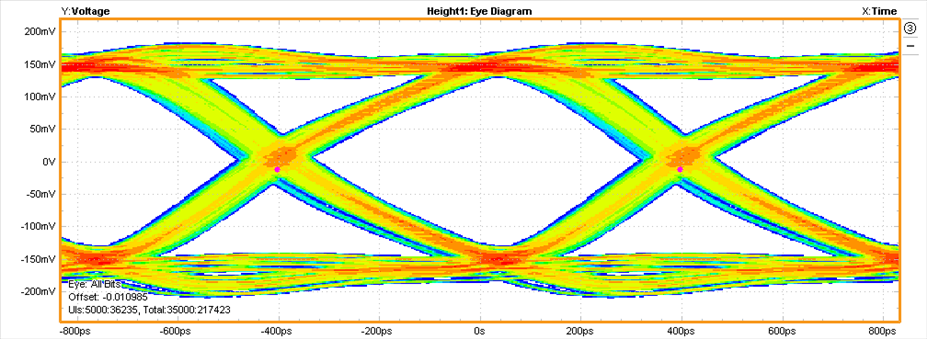
\includegraphics[width=0.8\linewidth]{sp-tpcelec-128Gbpseyesim.png}
\end{dunefigure}

%%%%%%%%%
\subsubsubsection{Commercial Off-the-shelf \dword{adc} Option}
\label{sec:fdsp-tpcelec-design-femb-alt-cots}

The \dword{sbnd} collaboration has been exploring the \dword{cots} \dword{adc} option 
for the \dword{tpc} readout electronics development since spring of 
2017~\cite{Chen:2018zic}. After a market survey, few candidate \dwords{adc} 
in \dword{sar} architecture were identified with 100\% cold yield. Starting in %Since 
July 2017, a lifetime study plan was developed to evaluate \dword{cots} 
\dword{adc} in two different phases: exploratory and validation. The 
lifetime study focused on the Analog Devices AD7274\footnote{AnalogDevices, AD7274\texttrademark{}, \url{https://www.analog.com/en/products/ad7274.html}.},
implemented in \dword{tsmc} \SI{350}{nm} \dword{cmos} technology, and has demonstrated  %given 
the optimum performance in cryogenic operation compared to other candidates. \fixme{check above -- something isn't optimum compared to something else; it's either better  or it's just plain optimum by itself. Maybe ``optimum performance in cryogenic operation, in contrast to other candidates''?}

During the exploratory phase, fresh samples of the \dword{cots} \dword{adc} 
AD7274 were stressed with higher than nominal operation voltage, e.g., 
\SI{5}{V}, while power consumption (current drawn) was monitored continuously. 
Periodically, the sample would be operated at nominal voltage (V$_{DD}$ = \SI{2.5}{V} 
and V$_{REF}$ = \SI{1.8}{V}) for a performance characterization test, where 
both the \dword{dnl} and \dword{inl} were monitored and analyzed in addition 
to the current. % monitoring. 
Stress test results were used to extrapolate the 
lifetime of the \dword{cots} \dword{adc}. We determined that a current drop 
of \num{1}\% on the V$_{DD}$ will be used as the degradation criterion for the lifetime 
study. In the validation phase, more devices were tested following the developed 
criteria to collect more data to validate what was learned in the exploratory phase.

The lifetime projection of the AD7274 \dword{adc} from the stress 
test with V$_{DD} >$ \SI{5}{V} is shown in Figure~\ref{fig:cotsadc-lifetime}. 
With the AD7274 operated at \SI{2.5}{V}, which is lower than the nominal 
\SI{3.6}{V} for the \SI{350}{nm} \dword{cmos} technology, the projected lifetime 
is more than than \num{1e6} years.

\begin{dunefigure}
[Lifetime projection of the \dword{cots} \dword{adc}]
{fig:cotsadc-lifetime}
{Lifetime projection of the \dword{cots} \dword{adc} AD7274 from the stress test 
with V$_{DD} >$ \SI{5}{V}. The current drop of 1\% on the V$_{DD}$ is used as 
degradation criterion. With nominal operation voltage of \SI{3.6}{V} for the 
\SI{350}{nm} \dword{cmos} technology, the lifetime is projected to be more 
than 100 years. For SBND and DUNE \dword{fd}, the AD7274 will be operated at 
\SI{2.5}{V} to add a further margin; the expected lifetime is more 
than \num{1e6} years.}
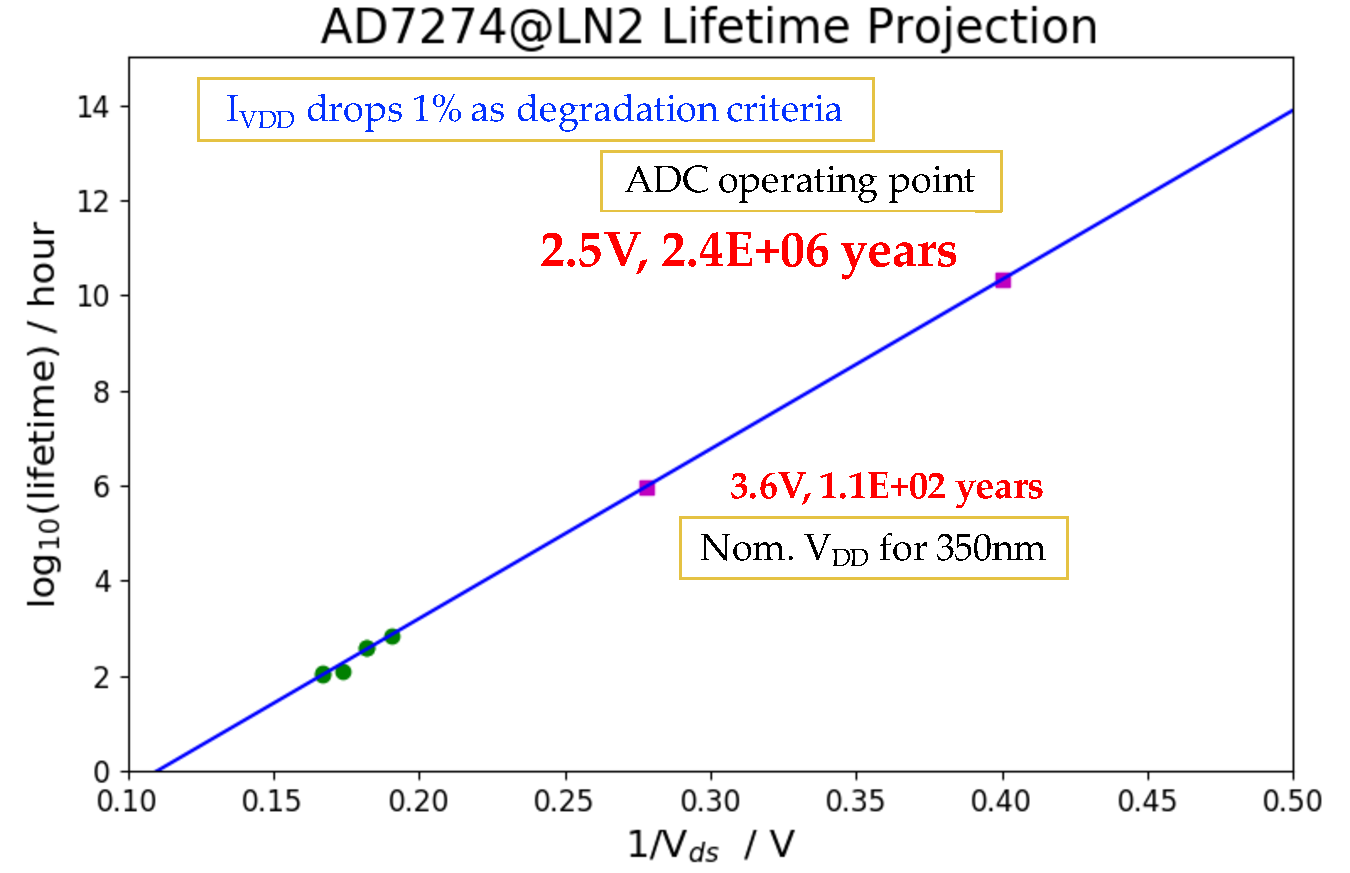
\includegraphics[width=0.8\linewidth]{sp-tpcelec-cotsadc-lifetime.pdf}
\end{dunefigure}

Based on the lifetime study of AD7274, a \dword{femb} with \dword{cots} 
\dword{adc} was developed and characterized for the \dword{sbnd} experiment. The 
integration test was carried out with 40\% \dword{apa} at \dword{bnl} and 
showed satisfactory noise performance in Figure~\ref{fig:cotsadc-fembenc}. 
The \dword{cots} \dword{adc} AD7274 serves as a backup solution for the 
\dword{dune} \dword{fd} \dword{tpc} readout electronics system. The current 
plan is to evaluate this \dword{adc} in the small \dword{tpc} 
\dword{iceberg} at \dword{fermilab}. Ten \dwords{femb} with \dword{cots} 
\dword{adc} are being produced and will be used to instrument \dword{iceberg} 
\dword{tpc} for system integration tests in the spring of 2019. 

\begin{dunefigure}
[Noise measurement of \dwords{femb} with \dword{cots} \dword{adc}]
{fig:cotsadc-fembenc}
{The noise measurement of \dwords{femb} with \dword{cots} \dwords{adc} 
mounted on the \num{40}\% APA at \dword{bnl}. The picture of the 
\dword{femb} is shown in the top left corner. The induction plane 
(\SI{4}{m} wire) has noise $\sim\SI{400}{e^-}$ with \SI{1}{$\mu$s} 
peaking time, and the collection plane (\SI{2.8}{m} wire) has noise 
$\sim\SI{330}{e^-}$ with \SI{1}{$\mu$s} peaking time.}
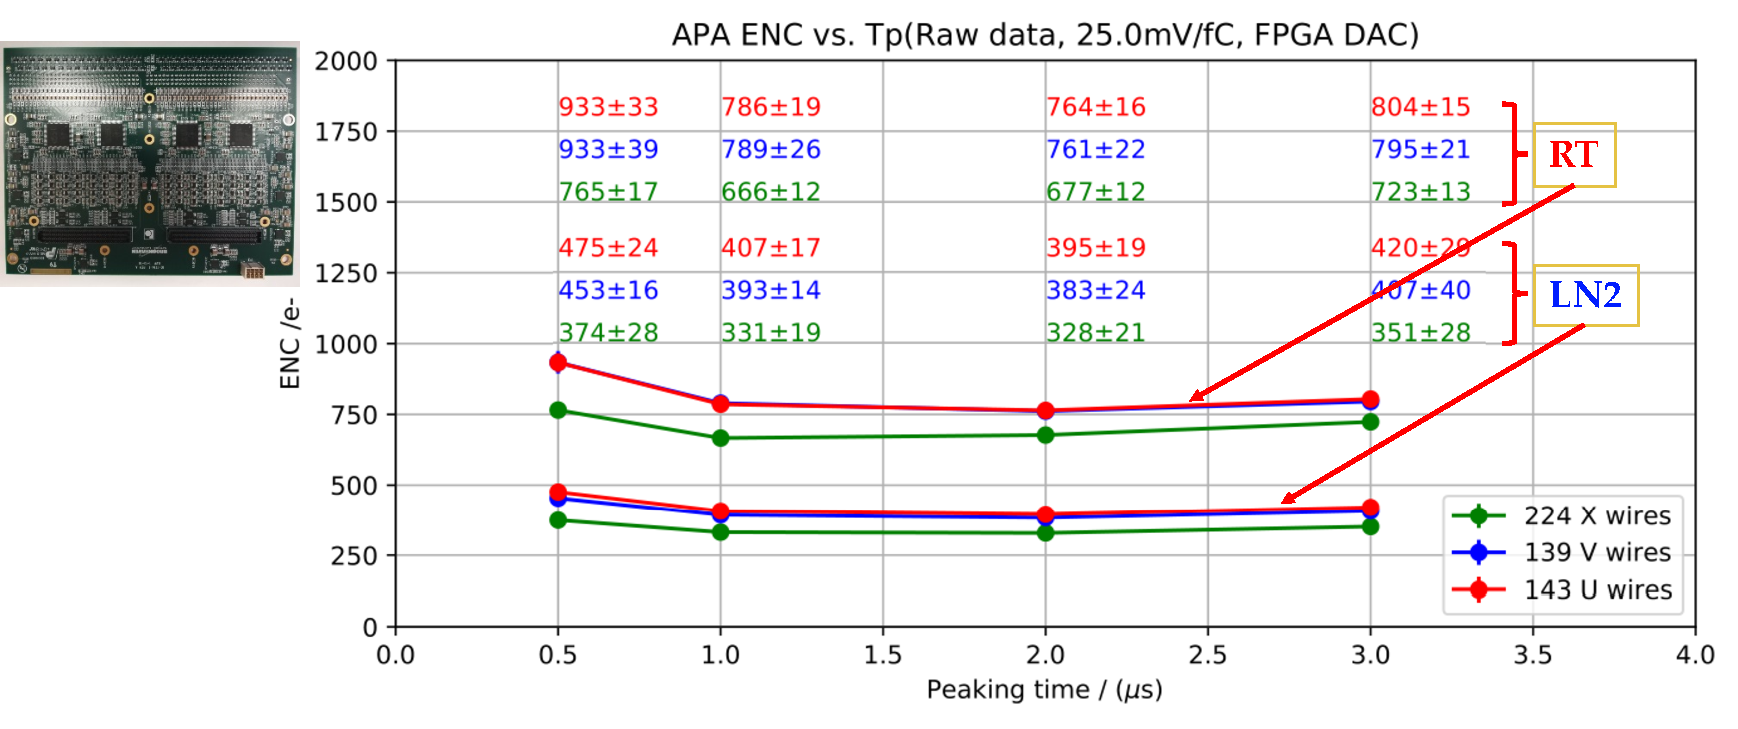
\includegraphics[width=0.99\linewidth]{sp-tpcelec-cotsadc-fembenc.pdf}
\end{dunefigure}


%%%%%%%%%
\subsubsubsection{CRYO Option}
\label{sec:fdsp-tpcelec-design-femb-alt-cryo}

The \dword{slac} \dword{cryo} \dword{asic} differs from the baseline 
three-chip design by combining the functions of an analog 
preamplifier, \dword{adc}, and data serialization along with %and 
transmission 
for \num{64}~wire channels into a single chip. It is based on a design 
developed for the \dword{nexo} experiment~\cite{nEXO} and differs from 
it only in the design of the preamplifier, which is modified for the 
higher capacitance of the \dword{dune} \dword{spmod} wires compared 
to the small pads of \dword{nexo}. The \dwords{femb} constructed using 
this chip would use only two \dwords{asic}, compared to the \num{18} 
(eight~\dword{fe}, eight~\dword{adc} and two~\dword{coldata}) needed 
in the baseline design. This drastic reduction in part count may 
significantly improve \dword{femb} reliability, reduce power, and reduce 
costs related to production and testing. 

Figure~\ref{fig:cryo-architecture} shows the overall architecture of 
the \dword{cryo} \dword{asic}, which is implemented in 
\SI{130}{nm} \dword{cmos}. It comprises two identical \num{32}-channel 
blocks. The current signal from each wire is amplified using a preamplifier 
with pole zero cancellation and an anti-alias fifth-order Bessel filter. 
Provisions are also made for injection of test pulses. Gain and peaking 
time are adjustable to values similar to those of the baseline design.

\begin{dunefigure}
[Overall architecture of the CRYO \dword{asic}.]
{fig:cryo-architecture}
{Overall architecture of the \dword{cryo} \dword{asic}.}
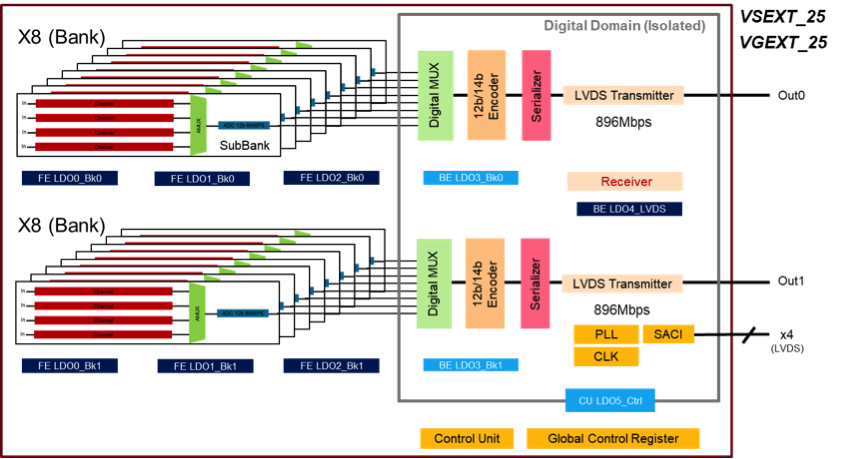
\includegraphics[width=0.8\textwidth]{sp-tpcelec-cryo-schematic.png}
\end{dunefigure}

The \dword{adc} uses \SI{8}{MHz} \dword{sar}, so four input channels are 
multiplexed onto a single \dword{adc}. The data serialization and transmission 
block uses a custom 12b/14b encoder, so \num{32} channels of \num{12}-bit, 
\SI{{\sim}2}{MHz} data can be transmitted with a digital bandwidth of 
only \SI{896}{Mbps}, which is significantly lower %less 
than the required bandwidth 
of the baseline, which is \SI{1.28}{Gbps}.

One key concern with mixed signal \dwords{asic} is the possibility of 
interference from the digital side causing noise on the very sensitive 
preamplifier. To avoid this interference, the \dword{cryo} design 
uses well established techniques for isolating the substrate; these are 
described in the literature~\cite{yeh} and %that 
have been successfully 
used in previous \dwords{asic}.

The infrastructure requirements for a \dword{cryo} \dword{asic}-based 
system are similar to those of the baseline option. However, in most 
cases, somewhat fewer resources are needed.
\begin{itemize}
\item{A single voltage is needed for the power supply. This is used to 
generate two supply voltages using internal voltage regulators.}
\item{The warm interface is different. Only a single clock is 
needed (\SI{56}{MHz}), and the configuration protocol is the 
\dword{saci}~\cite{SACI} rather than \dword{i2c}.}
\end{itemize}

The first iteration of the \dword{cryo} \dword{asic} design was 
submitted to MOSIS~\footnote{MOSIS\texttrademark{}, \url{https://www.mosis.com/}.} for fabrication in November 2018.  
The first prototypes were delivered at the end of January 2019. Simulation-based 
studies have already been performed; at \SI{0.8}{\micro\second} peaking 
time and an input capacitance of \SI{200}{pF} (similar to that expected 
in the \dword{spmod}), the noise level is approximately 
\num{500}\,e$^-$, similar to that expected with the 
baseline \dword{fe} and \dword{adc} \dword{asic} design in \dword{lar} 
with the same input capacitance.  The prototypes will first be tested in an existing 
test stand at \dword{slac}. Subsequent tests are planned for a small test 
\dword{tpc} at \dword{fermilab} and on an \dword{apa} in the \dword{pdsp} 
cold box; these test facilities are described in 
Section~\ref{sec:fdsp-tpcelec-qa-facilities}.

%%%%%%%%%%%%%%%%%%
\subsubsection{Procedure and Timeline for \dword{asic} Selection}
\label{sec:fdsp-tpcelec-design-femb-selection}

We are currently pursuing two different \dword{asic} designs and 
planning on qualifying the \dword{cots} \dword{adc} solution that 
will be used for the \dword{sbnd} experiment. %For the moment, we are planning 
we plan to continue developing both the three-\dword{asic} 
solution and the \dword{cryo} \dword{asic} for at least a second 
iteration before deciding which \dword{asic} solution to %use to construct 
implement in the \dword{dune} \dword{spmod}. % detector. 
This assumes that 
the \dwords{femb} populated with the first set of prototypes of 
the two kinds of \dwords{asic}, expected to become available in 
spring 2019, demonstrate a performance at least similar to that 
of the boards used for  \dword{pdsp}. We plan to review the results of the system tests and of the
component lifetimes discussed in Section~\ref{sec:fdsp-tpcelec-qa} in fall 
2019. 
In that review, we will also decide whether to change anything on 
the list of specifications %requirements 
for the \dwords{asic} and to further develop
the two custom \dword{asic} solutions, including fixing any 
issues found during the tests of the first version.  of the \dwords{asic}. 
We expect that the subsequent iteration
of the design, fabrication, and testing of the \dwords{asic} and
\dwords{femb} will take an additional twelve months. At the end 
of this process, when results from standalone tests of the
\dwords{asic} and system tests of the \dwords{femb} are
available, we should be in position to decide which \dword{asic}
solution to adopt. % for constructing the \dword{dune} \dword{sp} detector.

We have not yet completely identified the %exact 
criteria for the 
\dword{asic} selection. Performance in system tests will obviously
be one criterion, but we will need to consider reliability 
issues (which could favor the single-\dword{asic} solution 
that requires \dwords{femb} with fewer connections), power 
density (which could be less favorable to the \dword{cryo} solution),
and the costs and resources required during constructing 
and testing the \dwords{femb}. We plan to charge a committee
to draft a series of recommendations on how to select the
\dword{asic} and review the recommendations in fall
2019. Then we can %, before deciding 
decide on the second cycle of design for
\dwords{asic} and \dwords{femb}. Once the second cycle of design
and testing is complete, these recommendations will be used by the
committee charged with the final design review to suggest a
preferred option for the \dword{asic} solution. % for constructing the \dword{dune} \dword{sp} detector. 
The committee's recommendation %of the committee 
will then be passed to the \dword{dune} \dword{exb}, 
which is tasked with the final \dword{asic} decision.

%%%%%%%%%%%%%%%%%%%%%%%%%%%%%%%%%%%
\subsection{Infrastructure Inside the Cryostat}
\label{sec:fdsp-tpcelec-design-infrastructure}

Each \dword{femb} is enclosed in a mechanical \dword{ce} box 
to provide support, cable strain relief, and control of gas 
argon bubbles %in the \dword{lar} 
from the \dword{femb} attached 
to the lower \dword{apa} (which could in principle lead to 
discharge of the \dword{hv} system). The \dword{ce} box, 
illustrated in Figure~\ref{fig:ce-box}, is designed to make the 
electrical connection between the \dword{femb} and the \dword{apa} 
frame, as discussed %defined 
in Section~\ref{sec:fdsp-tpcelec-design-grounding}.
Mounting hardware inside the \dword{ce} box connects the ground plane 
of the \dword{femb} to the box casing. If argon bubbles %are formed 
form inside
the \dword{ce} box, they must get %these should be 
channeled through the two side
\dword{apa} frames, from where they would reach the top of the cryostat.
A test setup is being prepared at \dword{bnl} to measure the
maximum power that can be dissipated in \dword{lar} at a
depth equivalent to those of the \dwords{femb} installed on
the bottom \dword{apa}. Together with measurements of the
power consumption by new \dwords{asic}, this will inform
the need for further design of a system to collect any
argon bubbles and channel them through the \dword{apa} frames.

\begin{dunefigure}
[Prototype \dword{ce} box used in \dword{pdsp}.]
{fig:ce-box}
{Prototype \dword{ce} box used in \dword{pdsp}.}
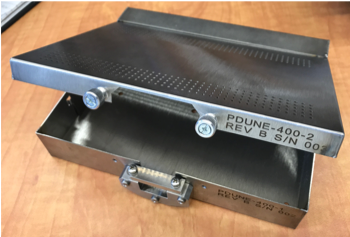
\includegraphics[width=0.45\linewidth]{sp-tpcelec-CEbox.png}
\end{dunefigure}

The \dword{ce} box casing is electrically connected to the 
\dword{apa} frame via the metal mounting hardware, called the 
Omega bracket (not shown in Figure~\ref{fig:ce-box}), and the 
input amplifier circuits are connected to the \dword{cr} board, 
which also terminate to ground at the \dword{apa} frame, as 
shown in Figure~\ref{fig:CR-board}. 
\fixme{the input amplifier circuits,  which also terminate to ground at the \dword{apa} frame, are connected to the \dword{cr} board...?}
As a backup, the casing is 
also connected to the \dword{apa} frame via a twisted conducting wire.

In addition to the \dword{ce} box and mounting hardware, cable trays 
for support and routing the cold cables will be installed in the 
cryostat. One set of cable trays, shown in Figure~\ref{fig:trays} 
(left column), will be attached to the upper \dword{apa} itself 
to hold the \dword{ce} and \dword{pd} cables. A different cable 
tray design, also shown in Figure~\ref{fig:trays} (right column), 
will support the \dword{ce} and \dword{pd} cables underneath the 
lower hanging \dword{apa}. A final set of cable trays will be 
installed inside the cryostat after the \dword{apa}s are 
fixed in their final location to support the cables as they are 
routed to the \dword{ce} and \dword{pd} feedthroughs.

\begin{dunefigure}
[Views of various cable and \dword{ce} cold boxes supports.]
{fig:trays}
{Side and end views of mechanical supports for the \dword{ce} 
Boxes on the upper (left column) and lower (right column) 
\dword{apa}s. Shown are the \dword{apa} cable trays in green and pink, 
the \dword{ce} boxes in dark gray, and the Omega brackets and mounting 
hardware between the \dword{ce} boxes and \dword{apa} frame in light gray.  
The \dword{ce} cables are shown in blue; the \dword{pd} cables are not shown.}
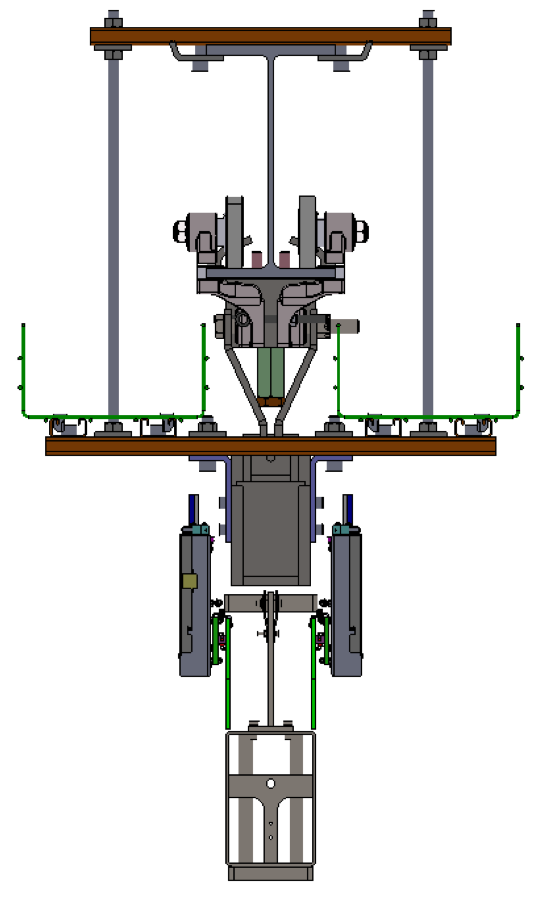
\includegraphics[width=0.38\linewidth]{sp-tpcelec-upper-tray2.png}
\hspace{5mm}
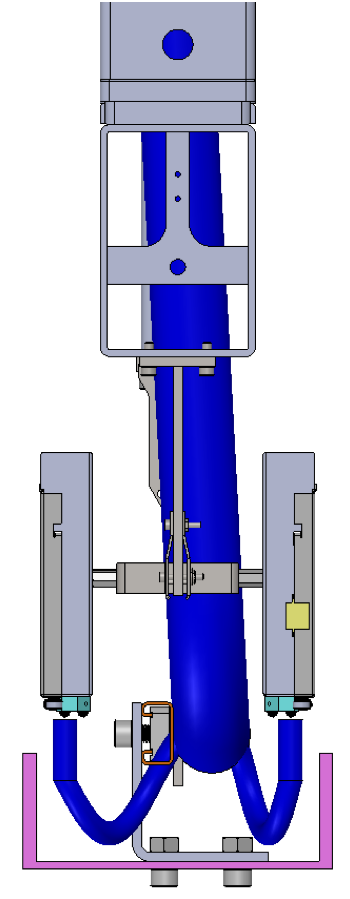
\includegraphics[width=0.25\linewidth]{sp-tpcelec-lower-tray2.png} \\
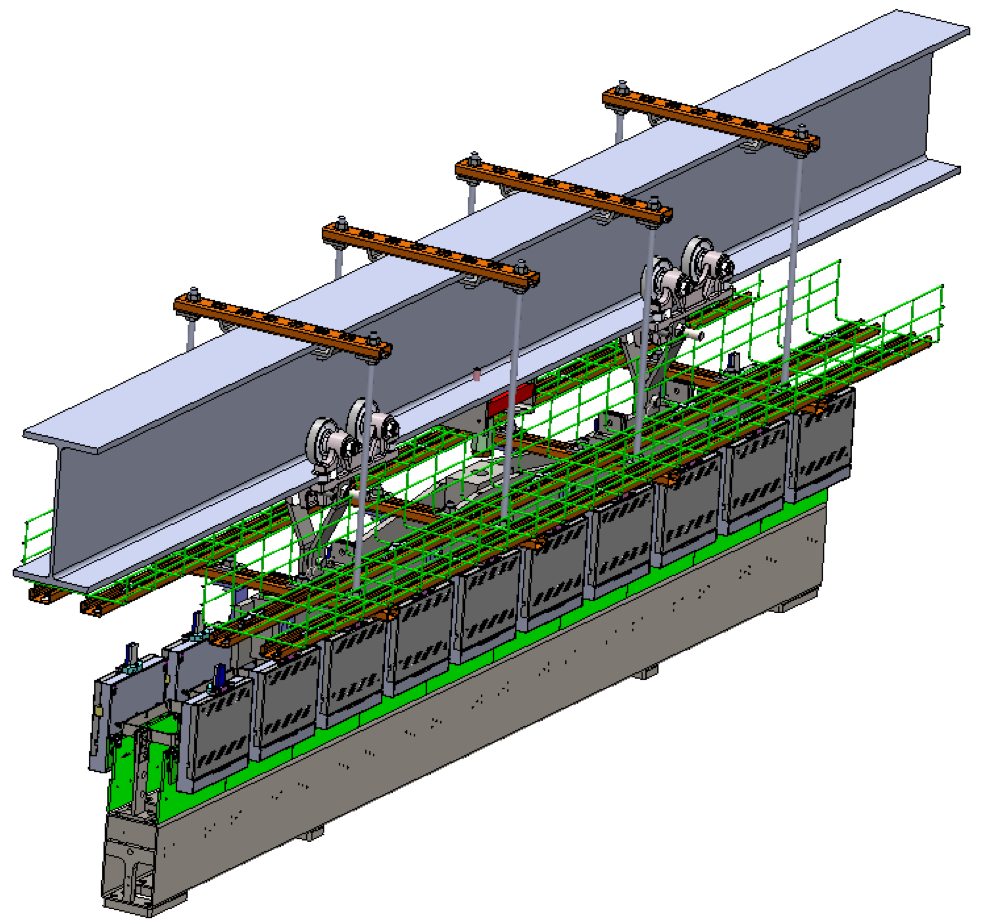
\includegraphics[width=0.32\linewidth]{sp-tpcelec-upper-tray1.png}
\hspace{5mm}
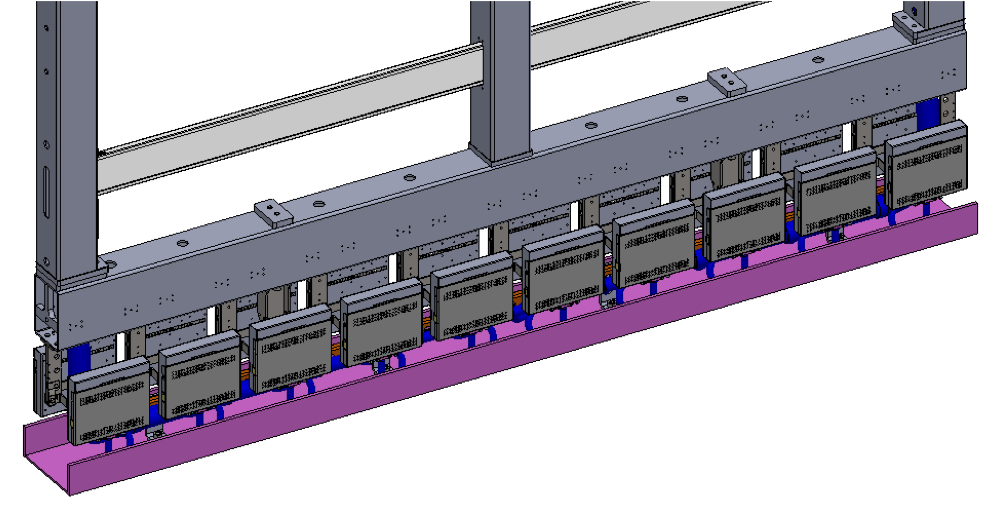
\includegraphics[width=0.4\linewidth]{sp-tpcelec-lower-tray1.png}
\end{dunefigure}



%%%%%%%%%%%%%%%%%%%%%%%%%%%%%%%%%%%
\subsection{Cold Cables and Cold Electronics Feedthroughs}
\label{sec:fdsp-tpcelec-design-ft}

All cold cables originating inside the cryostat connect to the outside 
warm electronics through \dwords{pcb} \fdth{}s installed in the signal 
flanges that are located on the cryostat roof. The \dword{tpc} data rate 
per \dword{apa}, with an overall multiplexing factor of \num{32} and 
\num{80} $\sim\SI{1}{Gbps}$ data channels per \dword{apa}, is 
sufficiently low that the \dword{lvds} signals can be driven over 
copper twin-axial transmission lines. Additional transmission lines 
are available to distribute \dword{lvds} clock signals and \dword{i2c} 
control information, which are transmitted at a lower bit rate.
Optical fiber is used externally from the \dwords{wib} on the signal 
flange to the \dword{daq} (see Chapter~\ref{ch:sp-daq}) and slow 
control systems (see Chapter~\ref{ch:sp-cisc}).

\begin{dunefigure}
[TPC \dword{ce} \fdth.]
{fig:tpcelec-signal-ft}
{TPC \dword{ce} \fdth. The \dwords{wib} are seen edge-on in the left 
panel and in an oblique side-view in the right panel, which also shows 
the warm crate for an \dword{spmod} in a cutaway view.}
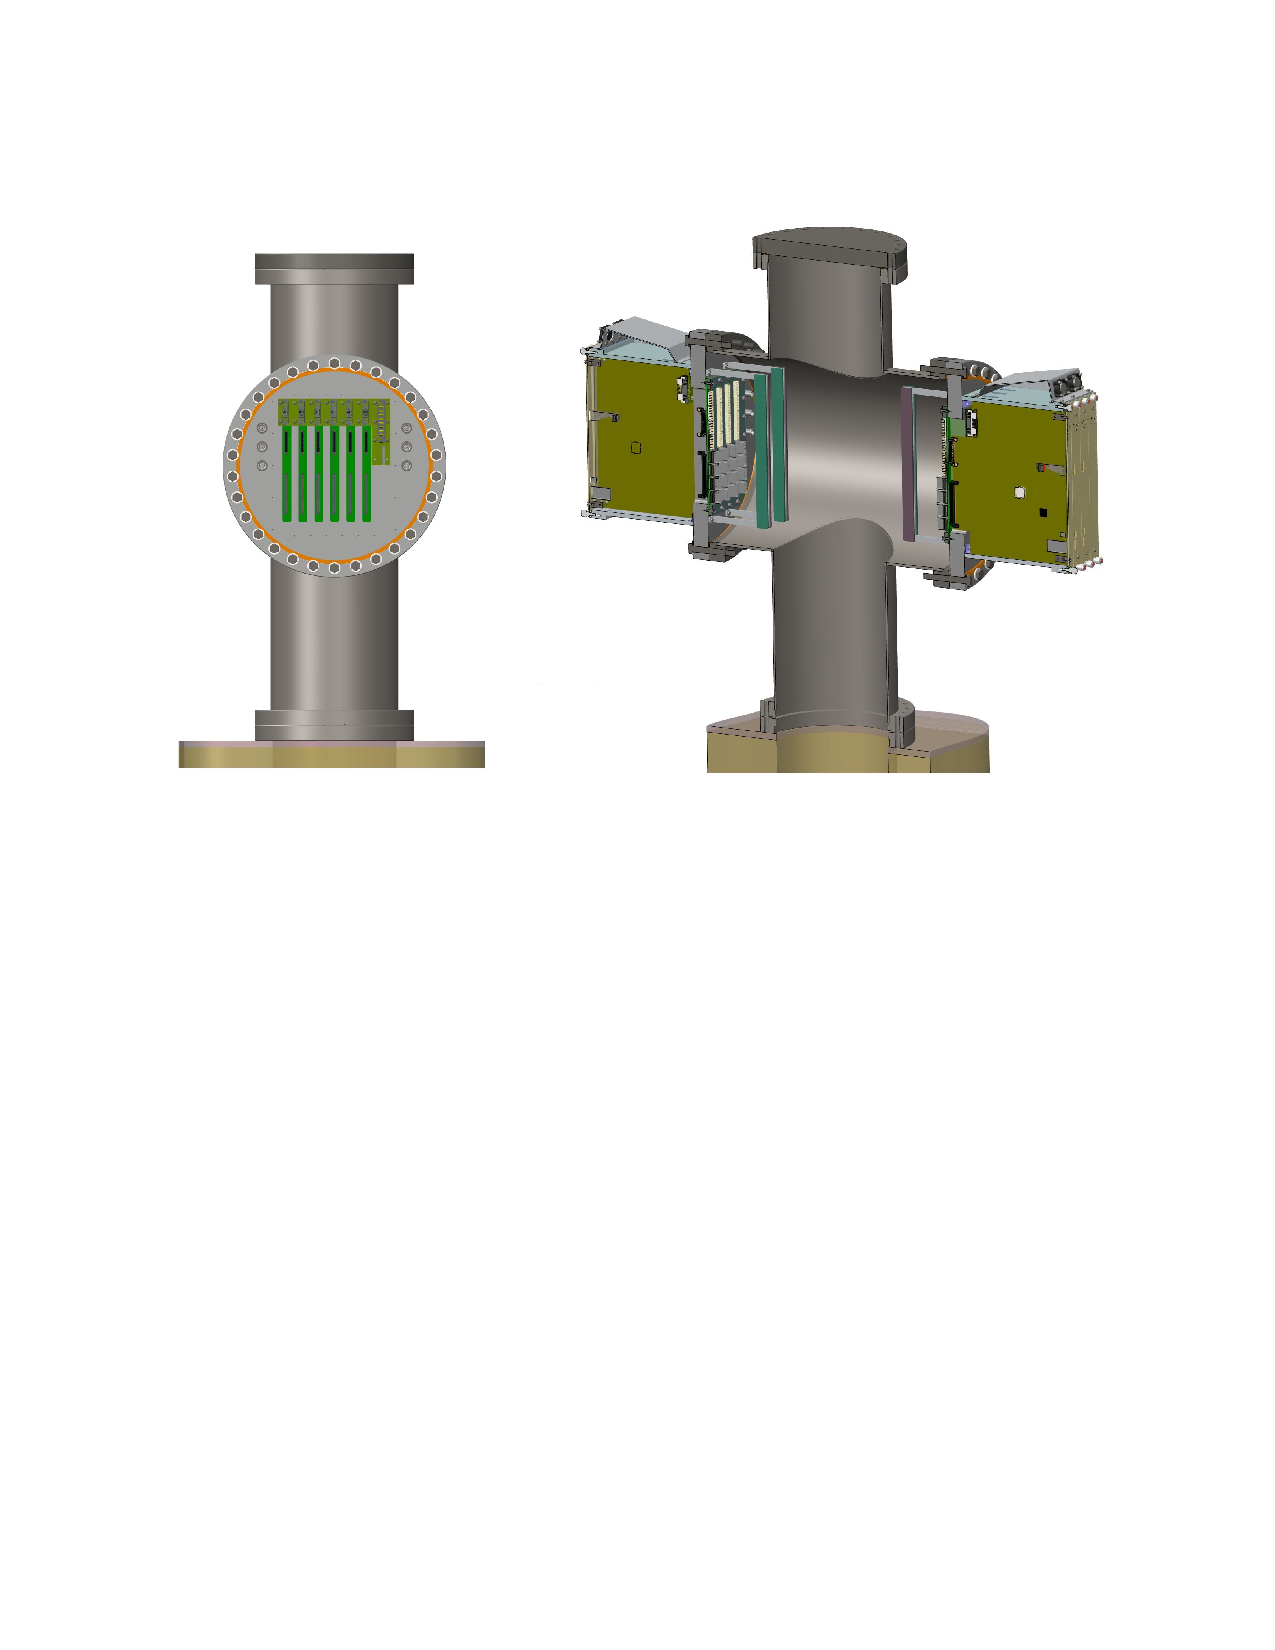
\includegraphics[width=0.9\linewidth]{sp-tpcelec-signal-FT.pdf}
\end{dunefigure}

The design of the signal flange includes a four-way cross spool 
piece, separate \dword{pcb} \fdth{}s for the \dword{ce} and 
\dword{pds} cables, and an attached crate for the \dword{tpc} 
warm electronics, as shown in Figure~\ref{fig:tpcelec-signal-ft}.
The wire bias voltage cables connect to standard \dword{shv} 
connectors machined directly into the \dword{ce} \fdth{}, ensuring 
no electrical connection between the wire bias voltages and other 
signals passing through the signal flange. Each \dword{ce} \fdth 
serves the bias, power, and digital I/O needs of one \dword{apa}.  

Data and control cable bundles send system clock and control signals 
from the signal flange to the \dword{femb} and stream the $\sim$\SI{1}{Gbps} 
high-speed data from the \dword{femb} to the signal flange. Each 
\dword{femb} connects to a signal flange via one data cable bundle, 
leading to \num{20} bundles between one \dword{apa} and one flange. 
In \dword{pdsp} each data bundle contains \num{12} low-skew twin-axial cables with a drain 
wire to transmit the following differential signals:
\begin{itemize}
\item four \SI{1.28}{Gbps} data (two from each \dword{coldata});
\item two \SI{64}{MHz} clocks (one input to each \dword{coldata});
\item two fast command lines (one input to each \dword{coldata});
\item three \dword{i2c}-like control lines (clock, data-in, and data-out); and
\item one multipurpose \dword{larasic} output (temperature, 
reference voltage, or analog test output).
\end{itemize}
For the \dword{dune} \dword{spmod} the total number of data and control cables could be 
reduced by doubling the data transmission speed to \SI{2.56}{Gbps}
and having only one link for each \dword{coldata} and/or by
sharing the clock and fast command lines between the two 
\dword{coldata} \dwords{asic}. This would reduce the number
of data and control cables to either ten or eight. In the
case of the \dword{cryo}, four cables are required to transmit
the data at \SI{896}{Mbps}, five cables are required for the
\dword{saci} protocol (three shared and one for each \dword{asic}
on the \dword{femb}), and in the current \dword{femb} prototype, 
two cables are used to transmit copies of the same \SI{56}{MHz}
clock. It is also possible in this case to reduce the 
number of data and control \fixme{cables?} by %either 
doubling the data transmission 
speed, %or by 
sharing the clock(s) between the two \dword{cryo} \dwords{asic}
on the \dword{femb}, or %by doing 
both.

The \dword{lv} power is passed from the signal flange to the 
\dword{femb} by bundles of \num{20}AWG twisted-pair wires. Half 
the wires are power feeds; the others are attached to the grounds 
of the input amplifier circuits, as described in 
Section~\ref{sec:fdsp-tpcelec-design-bias}.
For a single \dword{femb}, the resistance is measured to be 
$<\SI{30}{\milli\ohm}$ at room temperature ($<\SI{10}{\milli\ohm}$ 
at \dword{lar} temperature). Each \dword{apa} has a copper 
cross section of approximately \SI{80}{mm$^2$} with a 
resistance <\SI{1.5}{\milli\ohm} at room temperature or 
$<\SI{0.5}{\milli\ohm}$ at \dword{lar} temperature.
In the \dword{pdsp} design %there is 
a total of nine 
twisted-pair wires %that are used to 
bring power to the
\dwords{femb}, with four pairs of wires going to the analog
motherboard and five pairs connected to the mezzanine containing
the \dword{fpga}. Two pairs of wires (one for the motherboard,
and one for the mezzanine) %are used to 
provide a very low
current to the digital controls of the \dword{lv} converters 
(\SI{0.01}{A} at \SI{5}{V}). Six pairs of wires at %provide 
various voltages %that are used to 
provide power through the
\dword{lv} converters to the \dword{larasic} and the \dword{adc}
on the motherboard, and to the \dword{fpga} on the mezzanine.
The final wire pair is available for sending pulses to the
\dword{femb}. %It is hard to plan the exact number of 
%power connections required for \dword{dune}, since 
Measurements 
of power consumption for the new \dwords{asic} (\dword{coldadc}, 
\dword{coldata}, and \dword{cryo}) are not yet available, however 
it is conceivable that we can  reduce the number of twisted-pair
wires from %will be reduced from the current number of 
nine %down 
to at most seven, simply by removing the pair
reserved for sending pulses to the \dword{femb} and %by
%having a single line 
providing power to the digital 
controls of the \dword{lv} converters using a single line, most probably
because all the \dwords{asic} will fit on a single board. 
\fixme{what is most probable? Is it that we can reduce the number of wires (by these methods)  only if all the asics fit on a single board? Also check the two sentences below.}
%In the case that the \dword{cryo} is used the reduction
%could be even larger, 
Us of the \dword{cryo} would allow an even larger reduction, %as 
since the \dword{femb} may not need \dword{lv} regulators.  %may not
%be needed on the \dword{femb} 
And %fewer voltage levels are required, 
even if voltage sensing requires two pairs, fewer voltage levels are required. % would be needed for voltage sensing.

The bias voltages are applied to the $X$-, $U$-, and $G$-plane 
wire layers, three \dword{fc} terminations, and an electron diverter, 
as shown in Figure~\ref{fig:CR-board}. The voltages are supplied 
through eight \dword{shv} connectors mounted on the signal flange. 
RG-316 coaxial cables carry the voltages from the signal flange to 
a patch panel \dword{pcb} that includes noise filtering mounted on the top 
end of the \dword{apa}. From there, wire bias voltages are carried by single wires to 
various points on the \dword{apa} frame, including the \dword{cr} 
boards, a small \dword{pcb} mounted on or near the patch panel that 
houses a noise filter and termination circuits for the \dword{fc}  
voltages, and a small mounted board near the electron diverter 
that also houses wire bias voltage filters.

In Sections~\ref{sec:fdsp-apa-intfc-cables} and \ref{sec:fdsp-tpcelec-interfaces-apa}
we discuss the problem of routing the cold cables (data and control, power, and 
bias voltages) for the bottom \dword{apa} through the frames of both
the top and bottom \dword{apa}s. Routing tests were initially performed
with the \dword{pdsp} cable bundles (i.e., ten sets of 12 data and
control cables, ten sets of nine twisted-pair wires for power, and eight bias voltage
cables). To ensure successful cable routing %that the cables could be routed 
through the
\dword{apa} frame, the cross section of the side tubes was % has been
increased from %the original 
$\num{3}\times\SI{3}{in^2}$ %cross section 
to $\num{4}\times\SI{4}{in^2}$. Even with %the increased cross section 
this increase it was difficult to route the cable bundles for
ten \dwords{femb} through an \dword{apa} side tube. As discussed
above, the number of cables can be reduced slightly. 
\fixme{prev sentence doesn't seem to fit in}  Instead of
fabricating new cables \fixme{for protodune?}, we performed the routing tests with
nine sets of 12 data and control cables, nine sets of nine 
twisted-pair wires for power, and eight bias voltage cables.
This is to approximate the condition where there are ten sets
of 10 data and control cables, ten sets of eight twisted-pair
wires for power, and the same eight bias voltage cables. The
insertion test done in this conditions was succesful, once
a \SI{2.5}{in} diameter conduit was inserted inside the 
\dword{apa} frame to present a uniform cross section to
the cables and once the cables were restrained with a mesh
to facilitate the insertion in the conduit. The success of
these tests and the possibility of a further reduction in the
number of both data and control cables and of twisted-pair
wires used to bring power to the \dwords{femb} suggest
that there is a very high likelihood that it will be possible
to route the cold cables through the \dword{apa} frame.
\fixme{The above pgraph seems like too much detail for the overall design chapter. Could replace it with:} 

In Sections~\ref{sec:fdsp-apa-intfc-cables} and \ref{sec:fdsp-tpcelec-interfaces-apa}
we discuss the problem of routing the cold cables (data and control, power, and 
bias voltages) for the bottom \dword{apa} through the frames of both
the top and bottom \dword{apa}s. Routing tests were initially performed
with the \dword{pdsp} cable bundles, and even after increasing the 
the cross section of the side tubes from $\num{3}\times\SI{3}{in^2}$ 
to $\num{4}\times\SI{4}{in^2}$, routing was difficult. After understanding that we
could reduce the number of cables, we ran a second set of tests with fewer sets 
of cables (nine rather than ten sets of 12 data and control cables, nine rather than 
ten sets of nine twisted-pair wires for power, and eight bias voltage cables, as before).
This insertion test was successful, once
a \SI{2.5}{in} diameter conduit was inserted inside the 
\dword{apa} frame to present a uniform cross section to
the cables and the cables were restrained with a mesh. We expect that it will be possible
to route the cold cables through the \dword{apa} frame.

%%%%%%%%%%%%%%%%%%%%%%%%%%%%%%%%%%%
\subsection{Warm Interface Electronics}
\label{sec:fdsp-tpcelec-design-warm}

The warm interface electronics provide an interface between the 
\dword{ce}, \dword{daq}, timing, and slow control systems, including 
local power control at the flange and a real-time diagnostic readout. 
They are housed in the \dwords{wiec} attached directly to the \dword{ce} 
flange.  %The 
A \dword{wiec}, shown in Figure~\ref{fig:tpcelec-flange}, 
contains one \dword{ptc}, %power and timing card (\dword{ptc}),
 five %warm interface boards (
 \dwords{wib} %) 
 and a passive \dword{ptb}
that fans out signals and \dword{lv} power from the \dword{ptc} to the 
\dwords{wib}. The \dword{wiec} must provide Faraday-shielded housing, 
robust ground connections from the \dwords{wib} to the detector ground 
(Section~\ref{sec:fdsp-tpcelec-design-grounding}), and %only optical fiber 
links to the \dword{daq} and slow control. % to mitigate noise introduced at the \dword{ce} \fdth.
\fixme{reason for optical fiber should go elsewhere; too much info for intro pgraph}

\begin{dunefigure}
[Exploded view of the \dword{ce} signal flange for \dword{pdsp}.]
{fig:tpcelec-flange}
{Exploded view of the \dword{ce} signal flange for \dword{pdsp}.  
The design for the \dword{spmod} \dword{ce} 
signal flange will be very similar (with two \dword{ce} signal flanges per \fdth).}
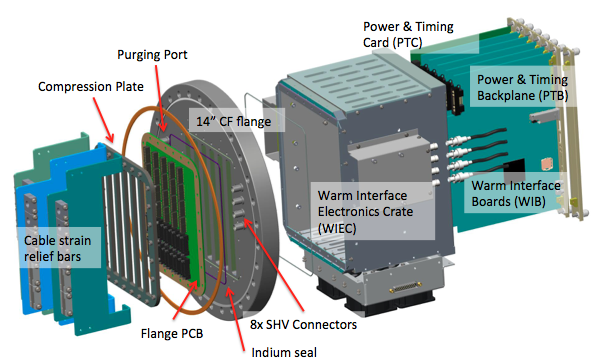
\includegraphics[width=0.9\linewidth]{sp-tpcelec-flange.png}
\end{dunefigure}

The \dword{wib} %is the interface between the \dword{daq} system and four \dwords{femb}. It 
receives the system clock and control signals from the
timing system and provides processing and fan-out of those signals to the four
\dwords{femb}. 
\fixme{above it says ``a passive \dword{ptb} that fans out signals and \dword{lv} power from the \dword{ptc} to the \dwords{wib}.'' What does the fanning out?}
%The \dword{wib} 
It also receives high-speed data signals from the four 
\dwords{femb} and transmits them to the \dword{daq} system over optical
fibers. The data signals are recovered onboard the \dword{wib} with commercial 
equalizers. The \dwords{wib} are attached directly to the \dword{tpc}
\dword{ce} \fdth on the signal flange. The \fdth board is a \dword{pcb} 
with connectors to the cold signal and \dword{lv} power cables fitted
between the compression plate on the cold side and sockets for
the \dword{wib} on the warm side. Cable strain relief for the cold cables is 
supported \fixme{provided?} from the back end of the \fdth.

The \dword{pdsp} \dword{ptc} provides a bidirectional fiber interface to the
timing system. The clock and data streams are separately fanned out to the 
five \dwords{wib} as shown in Figure~\ref{fig:tpcelec-wib-timing}. The 
\dword{ptc} fans the clocks out to the \dwords{wib} over the \dword{ptb}, which is a 
passive backplane attached directly to both. % the \dword{ptc} and \dwords{wib}. 
% The received clock on the \dword{wib} is separated into clock and
%data using a clock-data separator.
A clock-data separator on the \dword{wib} separates the received clock into clock and data. \fixme{very weird sentence} 
Timing endpoint firmware for receiving and transmitting %to receive and transmit
the clock is integrated into the \dword{wib} \dword{fpga} (the Altera 
Arria V\footnote{Altera Arria\texttrademark{} V, \url{https://www.altera.com/products/fpga/arria-series/arria-v/overview.html}.} was used for \dword{pdsp}). 
The \dword{spmod} timing system, described in Section~\ref{sec:sp-daq:design-timing}, 
is a further development of the \dword{pdsp} system and is expected to require nearly identical 
functionality \fixme{to function nearly identically?} at the \dword{wib} endpoint.

\begin{dunefigure}
[\dword{pdsp} PTC and timing distribution to the WIB and \dwords{femb}] % dwords for ptc and wib made this too long
{fig:tpcelec-wib-timing}
{\Dword{ptc} and timing distribution to the \dword{wib} and \dwords{femb} used in \dword{pdsp}.}
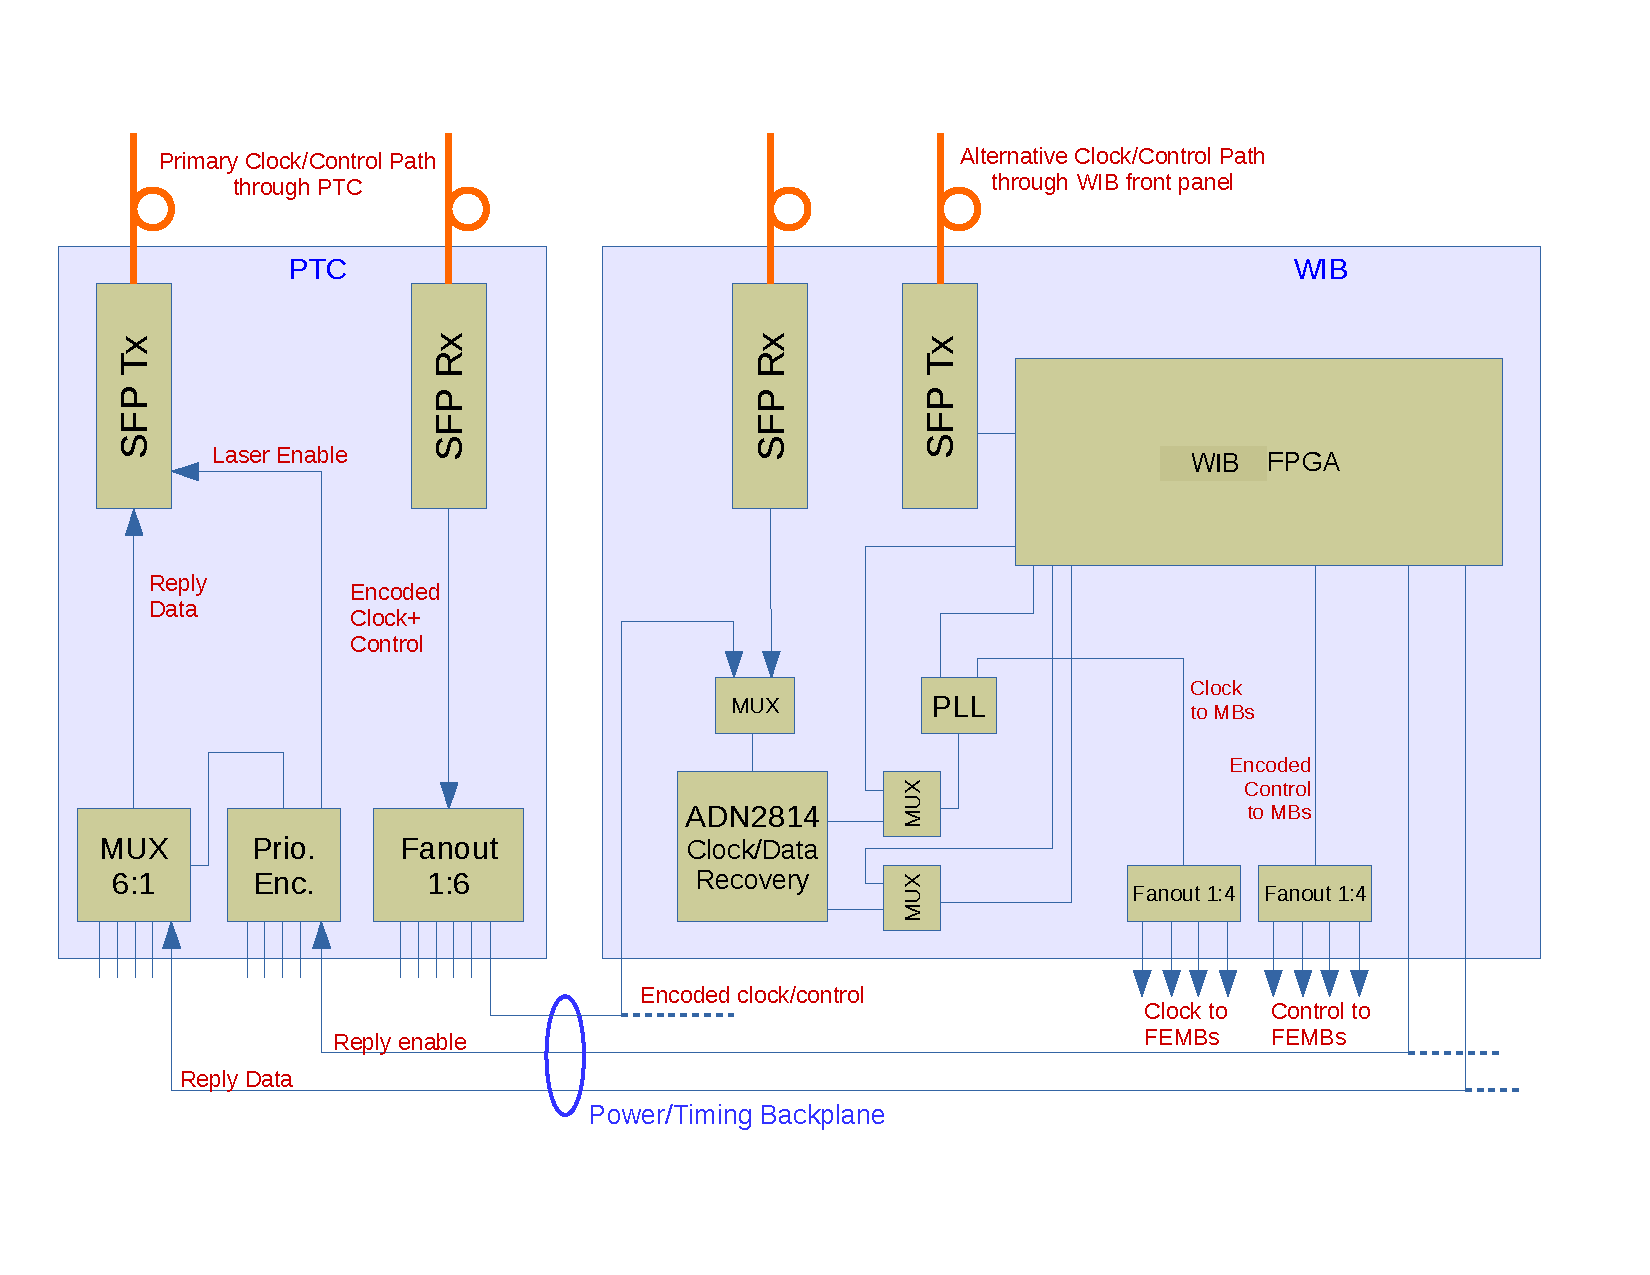
\includegraphics[width=0.75\linewidth]{sp-tpcelec-wib-timing-v2.pdf}
\end{dunefigure}

The \dword{ptc} %also 
receives \SI{48}{V} \dword{lv} power for all \dword{ce} %cold electronics 
connected through the \dword{tpc} signal flange: 
one \dword{ptc}, five \dwords{wib}, and \num{20}~\dwords{femb}. 
\fixme{confusing: clarify cold electronics vs warm side stuff}
The \dword{lv} power is then stepped down to \SI{12}{V} via 
a \dword{dc}-\dword{dc} converter onboard the \dword{ptc}. The output 
of the \dword{ptc} converters is filtered with a common-mode choke 
and fanned out on the \dword{ptb} to each \dword{wib}, which provides the 
necessary \SI{12}{V} \dword{dc}-\dword{dc} conversions and fans
the \dword{lv} power out to each of the cold \dwords{femb} supplied 
by that \dword{wib}, as shown in Figure~\ref{fig:tpcelec-wib-power}. 
The output of the \dword{wib} converters is further filtered by a 
common-mode choke. Most of the power drawn by a full flange is 
dissipated in the \dword{lar} by the cold \dword{femb}.

\begin{dunefigure}
[\dword{pdsp} \dword{lv} power distribution to the \dword{wib} and \dwords{femb}]
{fig:tpcelec-wib-power}
{\dword{lv} power distribution to the \dword{wib} and \dwords{femb} 
implemented for \dword{pdsp}. This will be modified for the 
\dword{spmod} to provide the required voltage or voltages 
depending on which \dwords{asic} are used on the \dwords{femb}. 
In particular, the voltages to the \dword{femb} \numrange{0}{3} 
will change as the \dword{pdsp} \dword{fpga} is replaced by \dword{coldata}. }
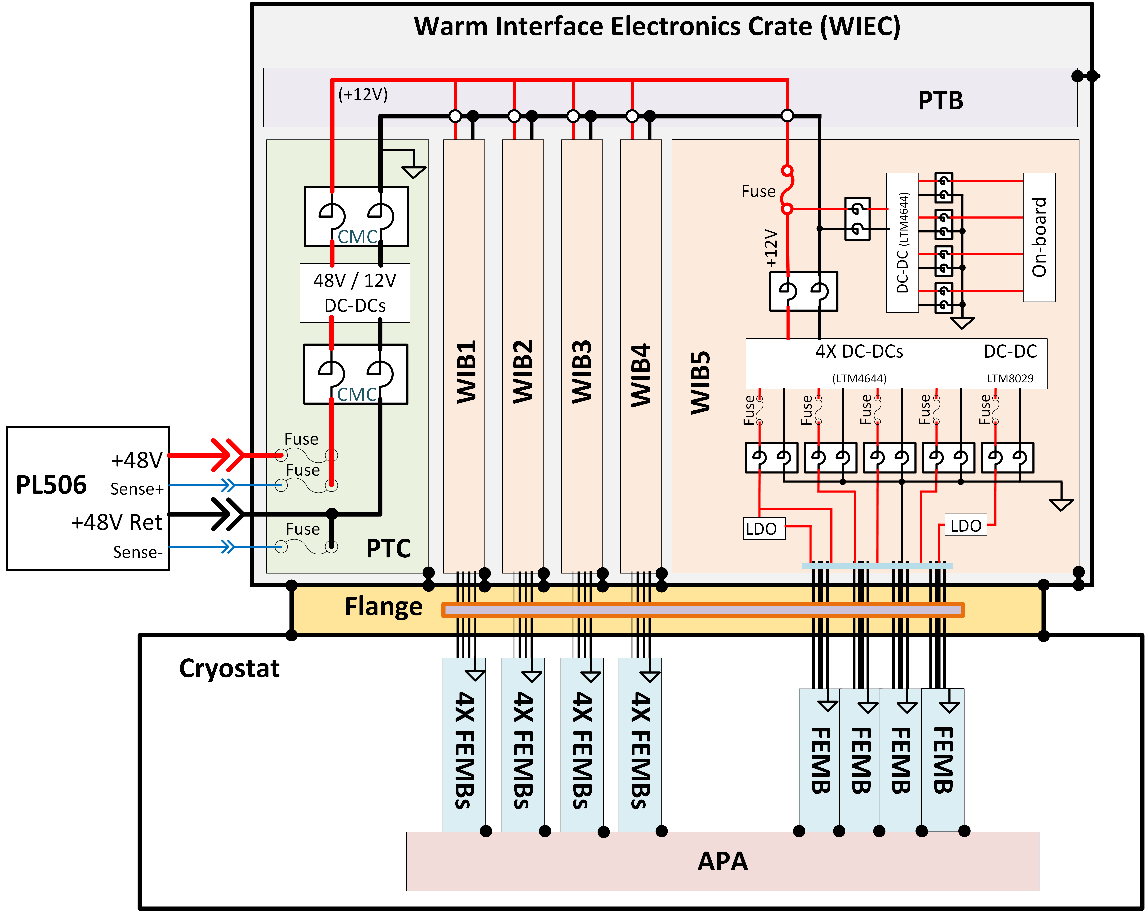
\includegraphics[width=0.65\linewidth]{sp-tpcelec-wib-power.pdf}
\end{dunefigure}

Because the \dwords{wib} can provide local power to the \dword{femb} 
and real-time diagnostic readout of all channels, each \dword{ce} 
system for each \dword{apa} is a complete, stand-alone readout unit. 
The \dwords{femb} and cold cables are shielded inside the cryostat, 
and the \dwords{wib} and \dword{ptc} are shielded inside the Faraday 
cage of the \dword{wiec}, with only shielded power 
cables and optical fibers connecting to external systems.

\begin{dunefigure}
[Warm interface board (\dword{wib})]
{fig:tpcelec-dune-wib}
{\dword{wib}. Note that front panel inputs include 
a LEMO connector and alternate inputs for \dword{lv} power and timing.}
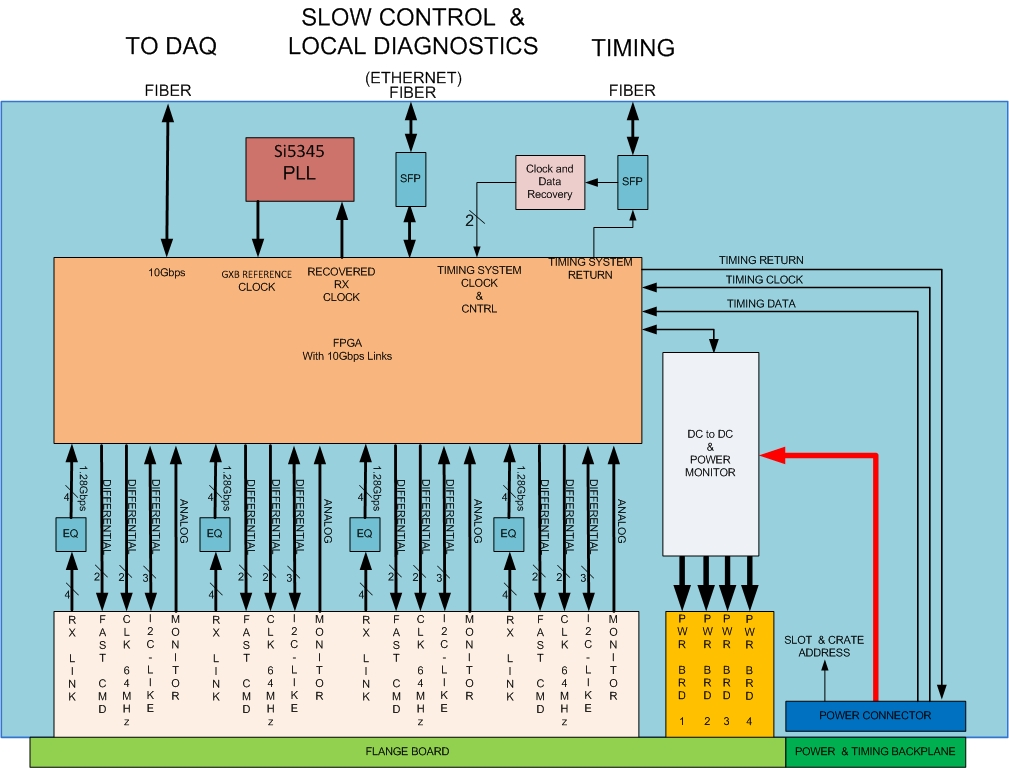
\includegraphics[width=0.8\linewidth]{sp-tpcelec-dune-wib.jpg}
\end{dunefigure}

As shown in Figure~\ref{fig:tpcelec-dune-wib}, the \dword{wib} can 
receive \dword{lv} power in the front panel and distribute it directly 
to the \dword{femb}, bypassing all \dword{dc}-\dword{dc} converters.
It can also receive the encoded system timing signals over bidirectional 
optical fibers on the front panel and process them using either
the on-board \dword{fpga} or clock synthesizer chip to provide the 
clock required by the \dword{ce}. The baseline \dword{asic} design 
currently uses 8b/10b encoding; if the \dword{slac} \dword{cryo} 
\dword{asic} is selected for the \dword{dune} \dword{spmod}, 
12b/14b encoding will be used instead of 8b/10b.

The \dword{fpga} on the \dword{wib} will have transceivers that can 
drive the high-speed data to the \dword{daq} system up to
\SI{10}{Gbps} per link, indicating that all data from
two \dwords{femb} (2$\times\SI{5}{Gbps}$) could be transmitted 
on a single link. The \dword{fpga} will have an additional 
Gbps Ethernet transceiver I/O based 
\fixme{I/O-based transceiver?} on the \SI{125}{MHz} clock, which 
provides real-time digital data readout to the slow control system.

%%%%%%%%%%%%%%%%%%
\subsection{Timing Distribution and Synchronization}
\label{sec:fdsp-tpcelec-design-timing}

The charge deposited on each wire of the \dword{apa}s installed 
in the \dword{dune} \dword{spmod} is digitized at a frequency of
$\sim\,\SI{2}{MHz}$, as discussed in 
Section~\ref{sec:fdsp-tpcelec-overview-requirements}. This requires
that the \dword{ce} be synchronized to a level of a few ns, which is
much smaller than the time difference between two charge samples.
This level of synchronization between the sampling time of different
\dwords{femb} contributes negligibly %gives a negligible contribution 
to the expected
resolution % of the measurement 
of the reconstructed space points measurement,
both in the \dword{apa} plane and along the drift distance.
The timing distribution and synchronization system for the %\dword{dune} 
\dword{spmod} is described in Section~\ref{sec:sp-daq:design-timing}.
Each \dword{wiec} has a bidirectional optical connection with the
timing system in the \dword{ptc}. Inside the \dword{ptc} the optical
signal from the timing system is converted, as discussed in the previous
section, to an electrical signal and distributed via the backplane to
the \dwords{wib} that constitute an endpoint for the timing distribution
system. Each \dword{wib} contains a standalone jitter-reducing \dword{pll} 
that %is used to 
forwards the clock to all the \dwords{femb}. The
\dword{fpga} contained inside the \dword{wib} implements the 
protocol~\cite{bib:docdb1651,bib:docdb11233}% that is needed 
for aligning
the phase of the clock at the endpoint of the distribution tree.

\fixme{Marco: the DAQ group should provide the information about 
the WIB synchronization. In \citedocdb{11233} it looks like this is 1 ns,
and I have asked David Cussans for confirmation.}

The timing distribution and synchronization system ensures that
all the \dwords{wib} are synchronized to within \SI{5}{ns}. %For
 The synchronization of the \dword{pdsp} \dwords{femb} relies on
the fact that all the cables connecting the \dwords{wib} to the
\dwords{femb} have approximately the same length (a length 
difference of \SI{0.5}{m} corresponds to a difference in the
sampling time of \SI{2.5}{ns}). We could use the same approach %could also be used 
for the \dword{dune} \dword{spmod}, correcting %inside the \dword{fpga} of the \dword{wib} 
for the top-bottom \dword{apa} cable length difference (corresponding to $\sim\,\SI{30}{ns}$) %in length between the cables for top and bottom \dword{apa}s
inside the \dword{fpga} of the \dword{wib}.  
%that corresponds to approximately \SI{30}{ns}. 
%This time difference could be measured for a sample of short and long cables 
We could measure the time difference for a sample of short and long cables prior to the installation of the \dwords{femb} on
the \dwords{apa}. %Using the cable lengths, 
Synchronizing
 the \dword{ce} with the \dword{pds} requires one (or two)
additional time constants that correspond to the transit 
time of the Fast Command sent from the \dword{wib} to
\dword{coldata} and from there to the \dword{coldadc},
which includes the propagation time along the cables
(\SIrange{35}{65}{ns}) plus the propagation time inside
the \dwords{asic}. This overall time constant  %that is ... below 
($<$\SI{100}{ns} in any case) could be obtained offline
from the data, but it represents at most a correction
of $\mathcal{O}(\SI{100}{\mu m})$ on the position of
a track along the drift distance. %Studies will be performed
%to understand whether the relative phase of the \dword{femb}
%and the \dword{wib} can be aligned more precisely by
%implementing a timer inside the \dword{fpga} in the
%\dword{wib} and measuring the transit time of a command
%sent to the \dword{femb} and of the corresponding return
%message.
We will implement a timer inside the \dword{wib}'s \dword{fpga} 
 and measure the transit time of a command
sent to the \dword{femb} and its corresponding return
message. This study will help us understand whether the 
relative phases of the \dword{femb}and the \dword{wib} 
can be aligned more precisely.

%It should be noted that 
The communication between the
\dword{wib} and the \dword{daq} backend is asynchronous
and %that 
the \num{64}-bit time-stamp is inserted in the data frame
in the \dword{wib}'s \dword{fpga}. %inside the \dword{wib}. 
%In the case of 
For the three-\dwords{asic} solution, the communication
from the \dword{femb} to the \dword{wib} is also
asynchronous and a \num{8}-bit time stamp is sent to
count the number of \dword{adc} samples from the last
``Sync'' signal, as discussed in Section~\ref{sec:fdsp-tpcelec-design-femb-coldata}.
This \num{8}-bit time stamp is used only for checking
the integrity of the data transmission between the 
\dword{femb} and the \dword{wib}. 

%One major difference between 
In contrast to the three-\dwords{asic} solution, %and 
in the \dword{cryo}-based \dwords{femb} solution %that
the communication between the \dword{femb} and 
\dword{wib} is entirely synchronous, using a \SI{56}{MHz} 
clock. In order to properly align the phase of the
\dword{adc} sampling for the top and bottom \dword{apa}s,
appropriate delays must be added to the sampling
command in the \dword{wib}'s \dword{fpga}. % inside the \dword{wib}.
%The considerations made above on the overall alignmentof 
The requirements listed above for synchronizing 
the \dword{ce} relative to the \dword{pds} remain
valid for this case. %also for the case of the \dword{cryo}-based \dwords{femb}.

\fixme{Marco: before submitting the TDR to the LBNC
we need to write something about the compatibility
of CRYO that uses a 56 MHz clock with the planned
62.5 MHz clock of the single phase detector.}


%%%%%%%%%%%%%%%%%%%%%%%%%%%%%%%%%%%
\subsection{Services on Top of the Cryostat}
\label{sec:fdsp-tpcelec-design-services}

A fully-loaded \dword{wib} (one \dword{wib} plus four \dwords{femb}) 
requires \SI{12}{V} and draws up to approximately \SI{4}{A}.  In 
\dword{pdsp} the full electronics for one \dword{apa} (one \dword{ptc}, 
five \dwords{wib}, and \num{20} \dwords{femb}) requires \SI{12}{V} and 
draws approximately \SI{20}{A}, for a total power of approximately 
\SI{240}{W}, as described in Section~\ref{sec:fdsp-tpcelec-design-warm}. 
The \dword{spmod} implementation should require less power because 
the \dword{fpga} will be replaced by the \dword{coldata} chips.

The \dword{lv} power is delivered at \SI{48}{V} to the \dword{ptc}, 
so each \dword{lv} power mainframe is chosen to bracket that value; 
each has roughly \numrange{30}{60}{V}, \SI{13.5}{A}, \SI{650}{W} 
maximum capacity per \dword{apa}. Using 10AWG cable, and assuming
a distance of \SI{20}{m} between the \dword{lv} power supplies 
that are situated on the detector mezzanine and the most distant
cryostat penetration for a row of \dword{apa}s, a \SI{0.8}{V} 
drop should occur along the cable with a required power of 
\SI{306}{W} out of \SI{650}{W} available. The power is almost entirely
dissipated inside the \dword{wiec} that is air-cooled, and
only a few watts are dissipated in the cables. Multiplying by
the total number of \dwords{wiec}, %there is
 less than \SI{1}{kW} of power %that 
is dissipated in the cabling system over the entire
surface of the cryostat.

Four wires are used for each module; two 10AWG, shielded, twisted-pair 
cables for the power and return; and two 20AWG, shielded, twisted-pair 
cables for the sense. The primary protection is the over-current 
protection circuit in the \dword{lv} supply modules, which is set 
higher than the \SI{20}{A} current draw of the \dword{wiec}. 
Secondary sense line fusing is provided on the \dword{ptc}.  
Tests are being performed in \dword{pdsp} to check which is the
best scheme for connecting the shields of the power cables. Most 
data was collected with the shield connected to ground on the 
power supply side, but tests are also planned with the shield
connected to ground on the \dword{wiec} side, and connected on both sides. %with both connections.

An additional \SI{18}{V} linear power supply will provide power to the 
cooling fans for the \dword{wiec}. It will be interlocked to the \SI{48}{V} 
power supplies, so the \dwords{wib} cannot be powered unless the cooling 
fans are operating. A \SI{10}{V} power supply will provide power to the four 
heating elements on each \dword{pd} and \dword{ce} flange.

Bias voltages for the \dword{apa} wire planes, the electron diverters, 
and the last \dword{fc} electrodes are generated by supplies that are 
the responsibility of the \dword{tpc} electronics consortium.  The 
current from each of these supplies should be very close to zero in 
normal operation. However, the ripple voltage must be carefully 
controlled to avoid injecting noise into the \dword{fe} electronics.  
RG-58 coaxial cables connect the wire bias voltages from the mini-crate 
to the standard \dword{shv} connectors machined directly into the 
\dword{ce} \fdth, so the \dword{lv} power and data connectors do not 
have electrical connections to wire bias voltages.

Optical fibers are used for all connections between the \dwords{wiec} %, 
%which act as Faraday-shielded boxes,  <<--- already said
and the \dword{daq} and slow 
control systems.  The \dword{wib} reports its onboard temperature 
and the current draw from each \dword{femb} to the slow control system, 
while the current draw for each \dword{apa} is monitored at the 
mainframe itself.

To support the electronics, fan, and heater power cables, as well 
as optical fibers on top of the cryostat, cable trays are installed
below the false flooring on top of the cryostat. These cable trays
run perpendicular to the main axis of the cryostat and connect the
three cryostat penetrations for one row of \dword{apa}s to the detector
mezzanine near the cryostat roof, as shown in Figure~\ref{fig:cryostat-roof}.
All the necessary \dword{lv} supplies and %, in addition to 
the bias
voltage supplies are installed in these racks. Patch panels for
the optical fiber plant used for the control and readout of the
detector are also installed in \fixme{on?} the detector mezzanine.

\begin{dunefigure}
[Services on top of the cryostat. ]
{fig:cryostat-roof}
{Services on top of the cryostat. The racks for the \dword{lv} power supplies are shown in blue.}
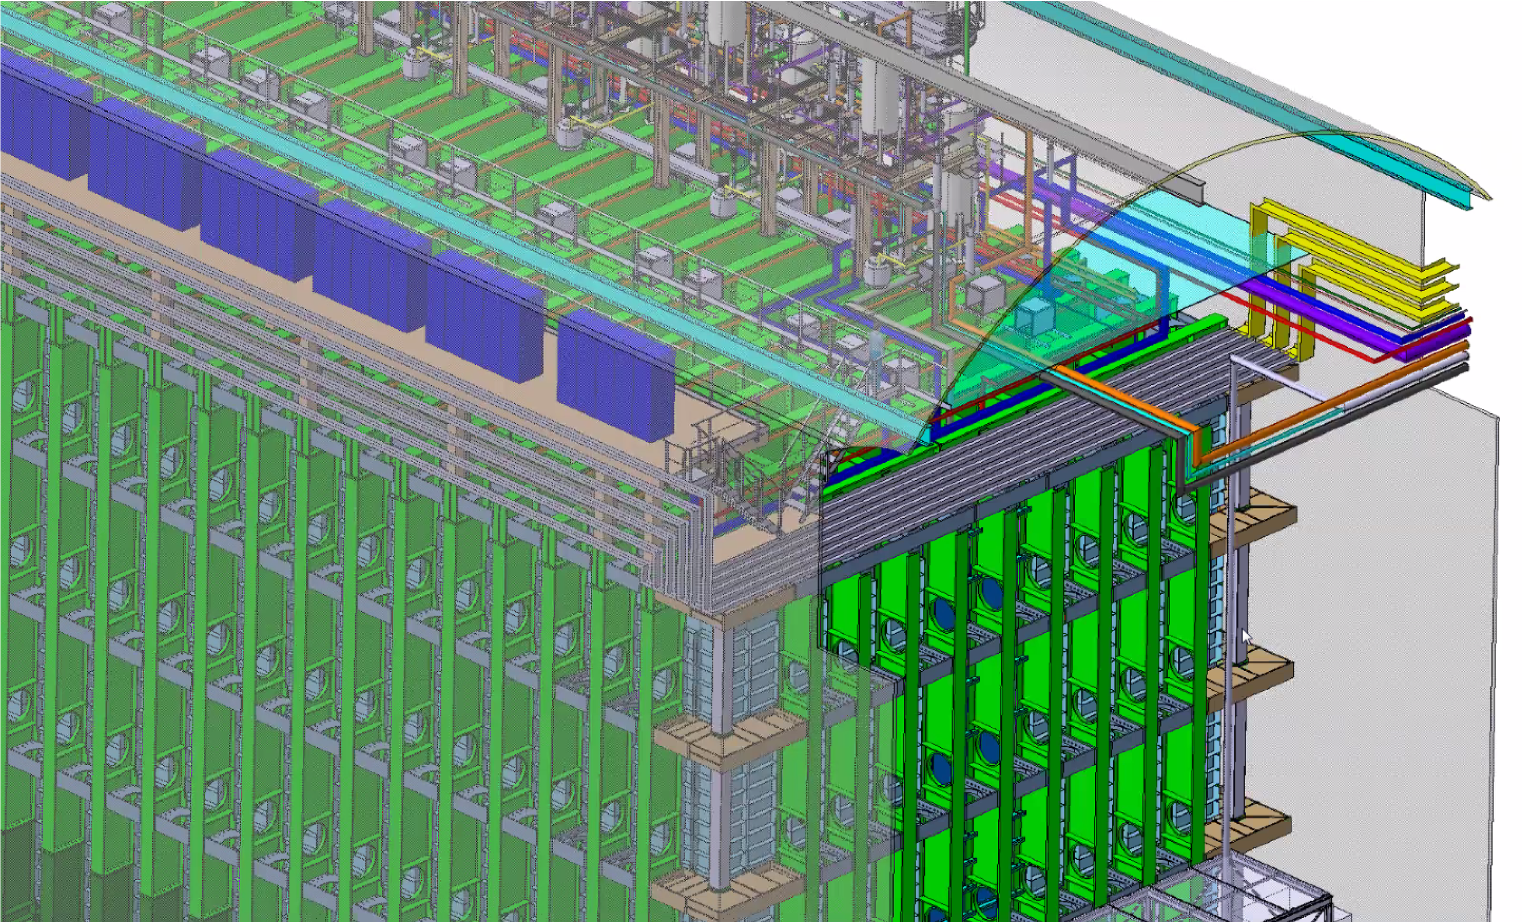
\includegraphics[width=0.9\linewidth]{sp-tpcelec-cryostat-top.png}
\end{dunefigure}

%%%%%%%%%%%%%%%%%%%%%%%%%%%%%%%%%%%
\subsection{Remaining Design and Prototyping Tasks}
\label{sec:fdsp-tpcelec-overview-remaining}

 \dword{pdsp} was %has been 
 built with multiple
goals, one of which was to demonstrate that the specifications
for \dword{dune} could be met with a design that would only require a simple
scale up of the detector size. The data collected with \dword{pdsp}
in fall 2018 has demonstrated that noise levels well below the target
of \SI{1000}{e$^-$} can be achieved in \lar, validating the
detector system design approach planned for the \dword{dune} \dword{spmod}.

%Despite the success of \dword{pdsp} there are multiple areas where
Still, additional design and prototyping work is required in several areas before %the
%beginning of the 
the start of \dword{spmod} construction, with differing levels of risk and engineering work, as estimated in Table~\ref{tab:SPCE:designstatus}. % \dword{dune} detector construction. 
%These design changes can be ordered depending on the risk and the amount of engineering that is required. 
\begin{comment}
At one end of the spectrum is the change of the
design of the cryostat penetration, that in \dword{pdsp} housed one
\dword{ce} and one \dword{pds} flange in a tee-shape. For \dword{dune}
there will be two \dword{ce} flanges in addition to the \dword{pds}
flange, arranged in the shape of a cross. The increase of the number
of flanges may require some structural reinforcement and additional
finite element analysis simulations to estimate the proper flow of
argon to avoid any back-diffusion of oxygen into the cryostat in case
of leaks on the flanges and to ensure that the temperature gradient
in the argon is acceptable. In cases like this it can be easily
argued that the amount of engineering required to finalize the
detector design for \dword{dune} is minimal compared to the work already
done for past \dword{lar} detectors, starting with \dword{microboone} and
other prototypes, and finishing with \dword{pdsp}. \end{comment}
%
For example, changing the number and arrangement of cryostat penetrations to accommodate 
 two \dword{ce} flanges in addition to the \dword{pds}
flange can be considered relatively minimal. It may require some structural reinforcement and additional \dword{fea} simulations to estimate the proper flow of
argon so as to avoid any back-diffusion of oxygen into the cryostat in case
of leaks on the flanges and to ensure an acceptable temperature gradient in the \lar.
%
\begin{comment}At the opposite
side of the spectrum is the \dword{asic} design, with the
development of \dword{coldata} and of a completely new \dword{adc}
that is being designed to address the shortcomings of the \dword{bnl}-designed
P1-\dword{adc}, non-linearities and stuck bits. In Table~\ref{tab:SPCE:designstatus}
we describe our estimate of the amount of work required to complete
the design and prototyping of the \dword{ce} detector components for
\dword{dune}. Later in this Section we analyze the risk that the design
and prototyping of these components could affect the \dword{dune} detector
construction schedule.\end{comment}
%
On the other hand, the \dword{asic} design, with the
development of \dword{coldata} and of a completely new \dword{adc} is more involved. 

\begin{dunetable}
[Status of the design of the different CE detector components]
{p{0.30\textwidth}p{0.15\textwidth}p{0.40\textwidth}}
{tab:SPCE:designstatus}
{Status of the design of the different CE detector components and expected
amount of engineering and prototyping required prior to construction.}
Component & Status & Expected work \\ \toprowrule
\dword{larasic} & Advanced & Fix minor issues in the design, port differential output from \dword{coldadc} design \\ \colhline
Commercial ADC & Complete & None \\ \colhline
\dword{coldadc} & \multicolumn{2}{l}{See text for details} \\ \colhline
\dword{coldata} & \multicolumn{2}{l}{See text for details} \\ \colhline
\dword{cryo} & \multicolumn{2}{l}{See text for details} \\ \colhline
\dword{femb} & Advanced & Experience with multiple prototypes, final design will follow the \dword{asic} selection \\ \colhline
Cold cables & Very advanced & Minor modifications, additional vendor qualification \\ \colhline
Cryostat penetrations & Advanced & Add \dword{ce} flange for bottom \dword{apa} \\ \colhline
\dword{wiec} & Very advanced & Add HEPA filter and hardware interlock system \\ \colhline
\dword{wib} & Advanced & Update design to use cheaper FPGA, modify \dword{femb} power \\ \colhline
\dword{ptc} & Very advanced & Add interface to interlock system \\ \colhline
Power supplies & Very advanced & Investigate possible additional vendors, rack arrangement \\ \colhline
Warm cables & Very advanced & Finalize cable layout, identify vendors \\ \colhline
Readout and control fiber plant & Very advanced & Finalize plant layout \\ \colhline
\end{dunetable}


The area that requires most work is that of the \dword{asic}s that are mounted
on the \dwords{femb}. The \dword{fe} \dword{asic} has already gone through eight design
iterations, the last three directly targeted for \dword{dune}, and has already been used, 
in one of its versions, for \dword{microboone} and for \dword{pdsp}, where it has reached the 
noise levels specified for the \dword{dune} \dword{spmod}. At least one additional design iteration is
required to address the issues observed during the \dword{pdsp} operations and
to implement a single-ended to differential converter to improve the interface
with the newly developed \dword{coldadc}. To ensure the success of the next 
design iteration we are investing in the development of appropriate transistor
models for operation in \lar, such that the saturation effect observed in 
\dword{pdsp} can be properly addressed first in simulation and then with improvements 
in design. It should be noted that so far approximate models, originally developed for 
the same \SI{180}{nm} technology, but with different design rules, have been used for 
the \dword{larasic} development, and therefore it should not be a surprise
that the \dword{fe} \dword{asic} may have limitations in some corner of the phase space.
The circuitry for the single-ended to differential converter has already been 
developed in the \SI{65}{nm} technology and needs to be ported to the \SI{180}{nm}
technology used for \dword{larasic}. We consider that appropriate measures have been
put in place to minimize the risk associated with the need of a further
prototyping iteration. Nevertheless, in Section~\ref{sec:fdsp-tpcelec-risks-design}
we consider a generic risk for a delay in the availability of \dword{asic}s and
argue that this delay would not have an impact on the beginning of \dword{dune} operations.

%The plan for the \dword{spmod} foresees the usage of 
The  \dword{spmod}  will likely need two additional custom design \dword{asic}s, one 
for the \dword{adc} and another for the data serialization, and the possibility of using a 
\fixme{third? or would this be the one asic that rules them all?} single 
\dword{asic} that combines these functionalities with that of the \dword{fe}. % It should be noticed that 
The \dword{sbnd}collaboration has demonstrated a 
 solution based on the use of a \dword{cots} \dword{adc} 
and  an \dword{fpga} for the data serialization, % has been demonstrated to work by the \dword{sbnd} collaboration, 
with further validation planned in spring 2019. 
As mentioned earlier, this solution %at this point 
is considered %as 
a fall-back solution for \dword{dune}. %Further verification work would be required to certify thatthe transceivers in the \dword{fpga} will meet the requirements of \dword{dune} for reliability in \lar. The c
Custom solutions for the \dwords{asic} are being developed to
simplify the \dword{femb} assembly and reduce the power dissipated by the
electronics in the \lar. %, which has consequences for the cryogenics and for the cross section of the cold cables and for the feedthroughs.

\fixme{I feel like I've already read all this next info}
The preferred solution for the \dword{adc} and the data serialization is based on two new 
\dword{asic}s, \dword{coldadc} and \dword{coldata}.
The first iteration of the \dword{coldadc} was submitted for fabrication
at the end of October 2018, and the chips were delivered in January 2019.
Test boards are being developed and results from the initial validation of the
chip functionality are expected for spring 2019. Although %Even if 
this is the first version
of the chip, we estimate that the design is already close to an advanced stage
for the following reasons:
\fixme{anne stopped here - it feels very repetitive. Maybe you can figure out what you still need to say here.}
\begin{itemize}
\item{An \dword{adc} with the same architecture has already been implemented by the
lead engineer of the \dword{bnl}-\dword{fnal}-\dword{lbnl} team that has designed the new \dword{coldadc}.
The new design is required to ensure operation in \lar, and the appropriate
models for the \SI{65}{nm} technology have been used, as discussed in
Section~\ref{sec:fdsp-tpcelec-design-femb-adc}.}
\item{The interfaces between the core of the \dword{adc} and \dword{larasic} on 
the input side and \dword{coldata} on the output side are entirely new.
These parts of the design have gone through an extensive verification
program, including \dword{spice} simulations of analog blocks,
mixed-mode simulations of the core \dword{adc} using the \dword{ams}
extensions of Verilog, and \dword{uvm} verification of 
all digital logic based on SystemVerilog. In addition, there are multiple 
input options that would allow the validation of the design of the core 
of the \dword{adc}, in the case that one of them does not function as designed.}
\item{For some blocks of the \dword{adc} (input buffers, voltage references) the
design includes multiple redundant options that can be selected during 
operation.}
\end{itemize}
If the tests of the new \dword{coldadc} in Spring 2019 are successful, the
estimate of the status of the design should be changed at least to the 
``Advanced'' status. One additional design iteration is planned before
the production, and as in the case of \dword{larasic}, plans can be made for a
further iteration without impacting the beginning of \dword{dune} operations.

We are also considering an alternative solution for the readout, where
the three \dword{asic}s are replaced with a single one, the \dword{cryo}
chip that is going through a development that is proceeding with a 
timeline similar to that of \dword{coldadc}. Also in this case the
chips from the first submission have been delivered in January 2019.
They will then undergo standalone tests
and later system tests on a timescale similar to that of \dword{coldadc}.
The \dword{cryo} chip is more complicated than \dword{coldadc},
since it implements the functionality of three \dword{asic}s into a
single one, and therefore its current design maturity status is
lower than that of \dword{coldadc}. Some of the design blocks of
\dword{cryo} are at a more advanced level: for example the control
and data transmission blocks have been reused from other \dword{asic}
designs from the \dword{slac} group, and the implementation of the \dword{fe} amplifier
is very similar to that of \dword{larasic}, except for the signal 
shaping. Depending on the results of the tests the status of the
\dword{cryo} design will evolve in a way similar to that of \dword{coldadc}.

The first complete prototype of \dword{coldata} will be submitted in 
March 2019, with the delivery of chips expected for June 2019.
The design of this first complete prototype builds on the success of
the first partial prototype (CDP1) that was fabricated and tested in 2018.
This first prototype included the control registers inside the 
\dword{asic}, the \dword{i2c} interface required to program and read-out
the status of these registers, the \dword{spi} interface required to
configure \dword{larasic}, the phase-lock loop required to generate
clocks internal to the chip, the data serializer, and a current-mode
line driver. The transition to the first complete prototype that
will be submitted in March 2019 and tested in Summer 2019
requires the addition of two interfaces to the \dword{coldadc} (\dword{uart}
and \dword{i2c}), an additional \dword{i2c} interface to allow programming two
\dword{coldata} \dword{asic}s on the same \dword{femb}, and the
addition of a line-driver with pre-emphasis required for operation
with long cables (up to \SI{23.5}{m}) in \lar. The same design and
validation methodology used for the CDP1 prototype and the \dword{coldadc}
is being used. This should guarantee that after the tests done in
Summer 2019 \dword{coldata} will reach the ``Advanced'' design 
status. 

There have already been multiple iterations of \dwords{femb} that
have been fabricated and tested and used for data taking in 
\dword{microboone} and in \dword{pdsp}. The \dword{sbnd} Collaboration
is starting the production of \dwords{femb} based on the commercial \dword{adc} and
\dword{fpga} solution. The design of the \dword{femb} needs to be adapted
for the different \dword{asic} solutions that are being considered
for \dword{dune}. This development is already ongoing, as system tests 
where the \dwords{femb} are connected to an \dword{apa} are part
of the qualification tests. The design status for the \dword{femb}
is already at the ``Advanced'' level, and it will reach the 
``Very advanced'' level at the time of the \dword{asic}
selection. At that point only minor modifications may be
required. 

The only other \dword{ce} detector components that do not yet
reach the ``Very advanced'' level are the cryostat penetrations, as
discussed above, and the \dword{wib}, where small
design changes will be done prior to production to use a more
modern and cheaper \dword{fpga}. Additional changes will be required to
the power distribution scheme, since the number of power lines
and the corresponding voltages will be reduced compared to
\dword{pdsp}. The transition to a more modern \dword{fpga} will allow 
more extensive data monitoring inside the \dword{wib}, but may
also require developing new software and porting the firmware
from one family of \dword{fpga}s to another. 

For all other detector components the estimate of the design
maturity is considered ``Very advanced'' based on the experience
gained with commissioning and operation of \dword{pdsp}. The 
cold signal cables will be modified to reduce the number of
connections and to address the issues observed with the connector
on the \dword{femb}. The design of the \dword{wiec} needs to
be modified to include \dword{hepa} filters to minimize the possible
damage from dust during the lifetime of the experiment at \dword{surf}.
The \dword{ptc} is going to be modified to add an interface to
the hardware interlocks of the detector safety system. For
cables and fibers on the top of the cryostat the only work that
remains to be done is the design of the actual cable plant, 
which will then fix the length of the cables. The arrangement
of power supplies in the racks on top of the cryostat is the
only other remaining design task. For many components the
qualification of additional vendors could also be considered
as part of value engineering, to reduce the risks of vendor
lock-in and to minimize costs. 

